% Options for packages loaded elsewhere
\PassOptionsToPackage{unicode}{hyperref}
\PassOptionsToPackage{hyphens}{url}
\PassOptionsToPackage{dvipsnames,svgnames,x11names}{xcolor}
%
\documentclass[
  letterpaper,
  DIV=11,
  numbers=noendperiod]{scrartcl}

\usepackage{amsmath,amssymb}
\usepackage{iftex}
\ifPDFTeX
  \usepackage[T1]{fontenc}
  \usepackage[utf8]{inputenc}
  \usepackage{textcomp} % provide euro and other symbols
\else % if luatex or xetex
  \usepackage{unicode-math}
  \defaultfontfeatures{Scale=MatchLowercase}
  \defaultfontfeatures[\rmfamily]{Ligatures=TeX,Scale=1}
\fi
\usepackage{lmodern}
\ifPDFTeX\else  
    % xetex/luatex font selection
\fi
% Use upquote if available, for straight quotes in verbatim environments
\IfFileExists{upquote.sty}{\usepackage{upquote}}{}
\IfFileExists{microtype.sty}{% use microtype if available
  \usepackage[]{microtype}
  \UseMicrotypeSet[protrusion]{basicmath} % disable protrusion for tt fonts
}{}
\makeatletter
\@ifundefined{KOMAClassName}{% if non-KOMA class
  \IfFileExists{parskip.sty}{%
    \usepackage{parskip}
  }{% else
    \setlength{\parindent}{0pt}
    \setlength{\parskip}{6pt plus 2pt minus 1pt}}
}{% if KOMA class
  \KOMAoptions{parskip=half}}
\makeatother
\usepackage{xcolor}
\setlength{\emergencystretch}{3em} % prevent overfull lines
\setcounter{secnumdepth}{-\maxdimen} % remove section numbering
% Make \paragraph and \subparagraph free-standing
\makeatletter
\ifx\paragraph\undefined\else
  \let\oldparagraph\paragraph
  \renewcommand{\paragraph}{
    \@ifstar
      \xxxParagraphStar
      \xxxParagraphNoStar
  }
  \newcommand{\xxxParagraphStar}[1]{\oldparagraph*{#1}\mbox{}}
  \newcommand{\xxxParagraphNoStar}[1]{\oldparagraph{#1}\mbox{}}
\fi
\ifx\subparagraph\undefined\else
  \let\oldsubparagraph\subparagraph
  \renewcommand{\subparagraph}{
    \@ifstar
      \xxxSubParagraphStar
      \xxxSubParagraphNoStar
  }
  \newcommand{\xxxSubParagraphStar}[1]{\oldsubparagraph*{#1}\mbox{}}
  \newcommand{\xxxSubParagraphNoStar}[1]{\oldsubparagraph{#1}\mbox{}}
\fi
\makeatother

\usepackage{color}
\usepackage{fancyvrb}
\newcommand{\VerbBar}{|}
\newcommand{\VERB}{\Verb[commandchars=\\\{\}]}
\DefineVerbatimEnvironment{Highlighting}{Verbatim}{commandchars=\\\{\}}
% Add ',fontsize=\small' for more characters per line
\usepackage{framed}
\definecolor{shadecolor}{RGB}{241,243,245}
\newenvironment{Shaded}{\begin{snugshade}}{\end{snugshade}}
\newcommand{\AlertTok}[1]{\textcolor[rgb]{0.68,0.00,0.00}{#1}}
\newcommand{\AnnotationTok}[1]{\textcolor[rgb]{0.37,0.37,0.37}{#1}}
\newcommand{\AttributeTok}[1]{\textcolor[rgb]{0.40,0.45,0.13}{#1}}
\newcommand{\BaseNTok}[1]{\textcolor[rgb]{0.68,0.00,0.00}{#1}}
\newcommand{\BuiltInTok}[1]{\textcolor[rgb]{0.00,0.23,0.31}{#1}}
\newcommand{\CharTok}[1]{\textcolor[rgb]{0.13,0.47,0.30}{#1}}
\newcommand{\CommentTok}[1]{\textcolor[rgb]{0.37,0.37,0.37}{#1}}
\newcommand{\CommentVarTok}[1]{\textcolor[rgb]{0.37,0.37,0.37}{\textit{#1}}}
\newcommand{\ConstantTok}[1]{\textcolor[rgb]{0.56,0.35,0.01}{#1}}
\newcommand{\ControlFlowTok}[1]{\textcolor[rgb]{0.00,0.23,0.31}{\textbf{#1}}}
\newcommand{\DataTypeTok}[1]{\textcolor[rgb]{0.68,0.00,0.00}{#1}}
\newcommand{\DecValTok}[1]{\textcolor[rgb]{0.68,0.00,0.00}{#1}}
\newcommand{\DocumentationTok}[1]{\textcolor[rgb]{0.37,0.37,0.37}{\textit{#1}}}
\newcommand{\ErrorTok}[1]{\textcolor[rgb]{0.68,0.00,0.00}{#1}}
\newcommand{\ExtensionTok}[1]{\textcolor[rgb]{0.00,0.23,0.31}{#1}}
\newcommand{\FloatTok}[1]{\textcolor[rgb]{0.68,0.00,0.00}{#1}}
\newcommand{\FunctionTok}[1]{\textcolor[rgb]{0.28,0.35,0.67}{#1}}
\newcommand{\ImportTok}[1]{\textcolor[rgb]{0.00,0.46,0.62}{#1}}
\newcommand{\InformationTok}[1]{\textcolor[rgb]{0.37,0.37,0.37}{#1}}
\newcommand{\KeywordTok}[1]{\textcolor[rgb]{0.00,0.23,0.31}{\textbf{#1}}}
\newcommand{\NormalTok}[1]{\textcolor[rgb]{0.00,0.23,0.31}{#1}}
\newcommand{\OperatorTok}[1]{\textcolor[rgb]{0.37,0.37,0.37}{#1}}
\newcommand{\OtherTok}[1]{\textcolor[rgb]{0.00,0.23,0.31}{#1}}
\newcommand{\PreprocessorTok}[1]{\textcolor[rgb]{0.68,0.00,0.00}{#1}}
\newcommand{\RegionMarkerTok}[1]{\textcolor[rgb]{0.00,0.23,0.31}{#1}}
\newcommand{\SpecialCharTok}[1]{\textcolor[rgb]{0.37,0.37,0.37}{#1}}
\newcommand{\SpecialStringTok}[1]{\textcolor[rgb]{0.13,0.47,0.30}{#1}}
\newcommand{\StringTok}[1]{\textcolor[rgb]{0.13,0.47,0.30}{#1}}
\newcommand{\VariableTok}[1]{\textcolor[rgb]{0.07,0.07,0.07}{#1}}
\newcommand{\VerbatimStringTok}[1]{\textcolor[rgb]{0.13,0.47,0.30}{#1}}
\newcommand{\WarningTok}[1]{\textcolor[rgb]{0.37,0.37,0.37}{\textit{#1}}}

\providecommand{\tightlist}{%
  \setlength{\itemsep}{0pt}\setlength{\parskip}{0pt}}\usepackage{longtable,booktabs,array}
\usepackage{calc} % for calculating minipage widths
% Correct order of tables after \paragraph or \subparagraph
\usepackage{etoolbox}
\makeatletter
\patchcmd\longtable{\par}{\if@noskipsec\mbox{}\fi\par}{}{}
\makeatother
% Allow footnotes in longtable head/foot
\IfFileExists{footnotehyper.sty}{\usepackage{footnotehyper}}{\usepackage{footnote}}
\makesavenoteenv{longtable}
\usepackage{graphicx}
\makeatletter
\newsavebox\pandoc@box
\newcommand*\pandocbounded[1]{% scales image to fit in text height/width
  \sbox\pandoc@box{#1}%
  \Gscale@div\@tempa{\textheight}{\dimexpr\ht\pandoc@box+\dp\pandoc@box\relax}%
  \Gscale@div\@tempb{\linewidth}{\wd\pandoc@box}%
  \ifdim\@tempb\p@<\@tempa\p@\let\@tempa\@tempb\fi% select the smaller of both
  \ifdim\@tempa\p@<\p@\scalebox{\@tempa}{\usebox\pandoc@box}%
  \else\usebox{\pandoc@box}%
  \fi%
}
% Set default figure placement to htbp
\def\fps@figure{htbp}
\makeatother
% definitions for citeproc citations
\NewDocumentCommand\citeproctext{}{}
\NewDocumentCommand\citeproc{mm}{%
  \begingroup\def\citeproctext{#2}\cite{#1}\endgroup}
\makeatletter
 % allow citations to break across lines
 \let\@cite@ofmt\@firstofone
 % avoid brackets around text for \cite:
 \def\@biblabel#1{}
 \def\@cite#1#2{{#1\if@tempswa , #2\fi}}
\makeatother
\newlength{\cslhangindent}
\setlength{\cslhangindent}{1.5em}
\newlength{\csllabelwidth}
\setlength{\csllabelwidth}{3em}
\newenvironment{CSLReferences}[2] % #1 hanging-indent, #2 entry-spacing
 {\begin{list}{}{%
  \setlength{\itemindent}{0pt}
  \setlength{\leftmargin}{0pt}
  \setlength{\parsep}{0pt}
  % turn on hanging indent if param 1 is 1
  \ifodd #1
   \setlength{\leftmargin}{\cslhangindent}
   \setlength{\itemindent}{-1\cslhangindent}
  \fi
  % set entry spacing
  \setlength{\itemsep}{#2\baselineskip}}}
 {\end{list}}
\usepackage{calc}
\newcommand{\CSLBlock}[1]{\hfill\break\parbox[t]{\linewidth}{\strut\ignorespaces#1\strut}}
\newcommand{\CSLLeftMargin}[1]{\parbox[t]{\csllabelwidth}{\strut#1\strut}}
\newcommand{\CSLRightInline}[1]{\parbox[t]{\linewidth - \csllabelwidth}{\strut#1\strut}}
\newcommand{\CSLIndent}[1]{\hspace{\cslhangindent}#1}

\KOMAoption{captions}{tableheading}
\makeatletter
\@ifpackageloaded{tcolorbox}{}{\usepackage[skins,breakable]{tcolorbox}}
\@ifpackageloaded{fontawesome5}{}{\usepackage{fontawesome5}}
\definecolor{quarto-callout-color}{HTML}{909090}
\definecolor{quarto-callout-note-color}{HTML}{0758E5}
\definecolor{quarto-callout-important-color}{HTML}{CC1914}
\definecolor{quarto-callout-warning-color}{HTML}{EB9113}
\definecolor{quarto-callout-tip-color}{HTML}{00A047}
\definecolor{quarto-callout-caution-color}{HTML}{FC5300}
\definecolor{quarto-callout-color-frame}{HTML}{acacac}
\definecolor{quarto-callout-note-color-frame}{HTML}{4582ec}
\definecolor{quarto-callout-important-color-frame}{HTML}{d9534f}
\definecolor{quarto-callout-warning-color-frame}{HTML}{f0ad4e}
\definecolor{quarto-callout-tip-color-frame}{HTML}{02b875}
\definecolor{quarto-callout-caution-color-frame}{HTML}{fd7e14}
\makeatother
\makeatletter
\@ifpackageloaded{caption}{}{\usepackage{caption}}
\AtBeginDocument{%
\ifdefined\contentsname
  \renewcommand*\contentsname{Table of contents}
\else
  \newcommand\contentsname{Table of contents}
\fi
\ifdefined\listfigurename
  \renewcommand*\listfigurename{List of Figures}
\else
  \newcommand\listfigurename{List of Figures}
\fi
\ifdefined\listtablename
  \renewcommand*\listtablename{List of Tables}
\else
  \newcommand\listtablename{List of Tables}
\fi
\ifdefined\figurename
  \renewcommand*\figurename{Figure}
\else
  \newcommand\figurename{Figure}
\fi
\ifdefined\tablename
  \renewcommand*\tablename{Table}
\else
  \newcommand\tablename{Table}
\fi
}
\@ifpackageloaded{float}{}{\usepackage{float}}
\floatstyle{ruled}
\@ifundefined{c@chapter}{\newfloat{codelisting}{h}{lop}}{\newfloat{codelisting}{h}{lop}[chapter]}
\floatname{codelisting}{Listing}
\newcommand*\listoflistings{\listof{codelisting}{List of Listings}}
\makeatother
\makeatletter
\makeatother
\makeatletter
\@ifpackageloaded{caption}{}{\usepackage{caption}}
\@ifpackageloaded{subcaption}{}{\usepackage{subcaption}}
\makeatother

\usepackage{bookmark}

\IfFileExists{xurl.sty}{\usepackage{xurl}}{} % add URL line breaks if available
\urlstyle{same} % disable monospaced font for URLs
\hypersetup{
  pdftitle={U.S. National Park Visit Data (1979-2023)},
  pdfauthor={Melanie Walsh and Os Keyes},
  colorlinks=true,
  linkcolor={blue},
  filecolor={Maroon},
  citecolor={Blue},
  urlcolor={Blue},
  pdfcreator={LaTeX via pandoc}}


\title{U.S. National Park Visit Data (1979-2023)}
\author{Melanie Walsh and Os Keyes}
\date{2024-06-01}

\begin{document}
\maketitle


\section{Data Essay}

\subsection{Introduction}\label{introduction}

This dataset contains the number of visits, per year, to each of the
current
\href{https://en.wikipedia.org/wiki/List_of_national_parks_of_the_United_States\#National_parks}{63
National Parks} administered by the United States National Park Service
(NPS), from 1979 to 2023. The NPS also collects visitation and use data
about other park units, such as
\href{(https://www.nps.gov/aboutus/national-park-system.htm)}{national
battlefields, national rivers, and national monuments}. However,
information about other park units is not included in this particular
dataset.

\begin{tcolorbox}[enhanced jigsaw, title={Brief Survey}, opacityback=0, bottomtitle=1mm, left=2mm, coltitle=black, opacitybacktitle=0.6, breakable, arc=.35mm, colframe=quarto-callout-tip-color-frame, toprule=.15mm, rightrule=.15mm, colback=white, colbacktitle=quarto-callout-tip-color!10!white, leftrule=.75mm, toptitle=1mm, titlerule=0mm, bottomrule=.15mm]

If you use our materials in your class or another setting, we would love
to \href{https://forms.gle/yJpQscUH9k9Rn4Qy9}{hear about it}!

\end{tcolorbox}

\begin{tcolorbox}[enhanced jigsaw, title={View Summary of Columns}, opacityback=0, bottomtitle=1mm, left=2mm, coltitle=black, opacitybacktitle=0.6, breakable, arc=.35mm, colframe=quarto-callout-note-color-frame, toprule=.15mm, rightrule=.15mm, colback=white, colbacktitle=quarto-callout-note-color!10!white, leftrule=.75mm, toptitle=1mm, titlerule=0mm, bottomrule=.15mm]

\begin{Shaded}
\begin{Highlighting}[]
\NormalTok{//|echo: false}
\NormalTok{viewof selectedColumns}
\NormalTok{viewof dataSummaryView}
\end{Highlighting}
\end{Shaded}

\end{tcolorbox}

\begin{tcolorbox}[enhanced jigsaw, title={Creative Commons License}, opacityback=0, bottomtitle=1mm, left=2mm, coltitle=black, opacitybacktitle=0.6, breakable, arc=.35mm, colframe=quarto-callout-tip-color-frame, toprule=.15mm, rightrule=.15mm, colback=white, colbacktitle=quarto-callout-tip-color!10!white, leftrule=.75mm, toptitle=1mm, titlerule=0mm, bottomrule=.15mm]

This work is licensed under CC BY 4.0

\end{tcolorbox}

The National Park datasets included here are drawn from data published
by the U.S. NPS, and most (but not all) of the contextual information is
drawn from material published by the NPS.

We decided to publish this version of the data, along with our own
synthesized documentation and narrative, because the original data is
made available in an \href{https://irma.nps.gov/Stats/}{NPS data portal}
that is relatively hard to find and to use, and the documentation is
distributed across many different web pages, PDFs, and other documents.
(The NPS has created an interactive
\href{https://www.nps.gov/subjects/socialscience/visitor-use-statistics-dashboard.htm}{Microsoft
Power BI dashboard} to help users explore the data more easily.)

The datasets were curated and published by Melanie Walsh, and the data
essay was written by Melanie Walsh and Os Keyes.

\subsection{History}\label{history}

A national park is an area of land that a country's government deems
important enough to officially protect, preserve, and make available to
the public. There are thousands of national parks around the world (some
of which are featured in the Netflix documentary,
\href{https://www.netflix.com/title/81086133}{``Our Great National
Parks,''} narrated by former President Barack Obama).

In the United States, the very first National Park---Yellowstone
National Park, in Wyoming---was signed into law in 1872 by President
Ulysses S. Grant.

\begin{figure}

\centering{

\pandocbounded{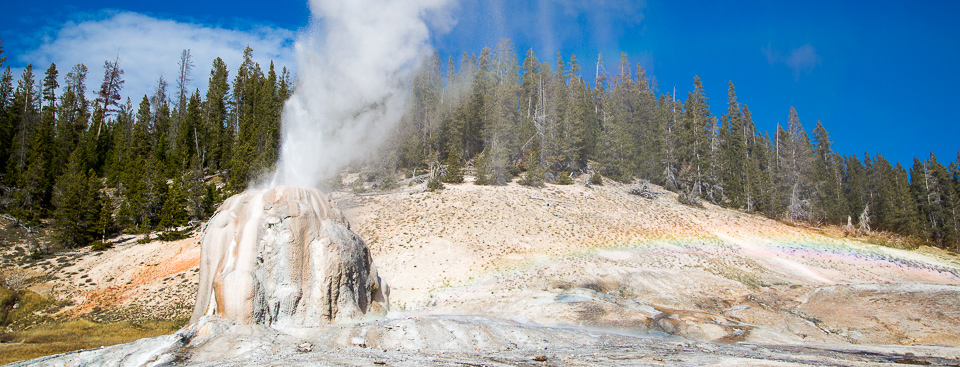
\includegraphics[keepaspectratio]{index_files/mediabag/ndh-yell-9306.jpg}}

}

\caption{\label{fig-yellowstone}Old Faithful, the most famous geyser of
the whopping \textasciitilde500 geysers at Yellowstone National Park.
Photo credit:
\href{https://www.nps.gov/yell/planyourvisit/exploreoldfaithful.htm}{NPS/Neal
Herbert}.}

\end{figure}%

Over the next several decades, a handful of other parks---such as
Sequoia (1890), Yosemite (1890), Mount Rainier (1899), and Crater Lake
(1902)---joined the system, too.

\begin{tcolorbox}[enhanced jigsaw, title=\textcolor{quarto-callout-tip-color}{\faLightbulb}\hspace{0.5em}{What is the most recent National Park?}, opacityback=0, bottomtitle=1mm, left=2mm, coltitle=black, opacitybacktitle=0.6, breakable, arc=.35mm, colframe=quarto-callout-tip-color-frame, toprule=.15mm, rightrule=.15mm, colback=white, colbacktitle=quarto-callout-tip-color!10!white, leftrule=.75mm, toptitle=1mm, titlerule=0mm, bottomrule=.15mm]

The most recently added National Park is
\href{https://www.nps.gov/neri/index.htm}{New River Gorge National Park}
in West Virginia. It was designated in 2020.

\end{tcolorbox}

\begin{figure}

\centering{

\pandocbounded{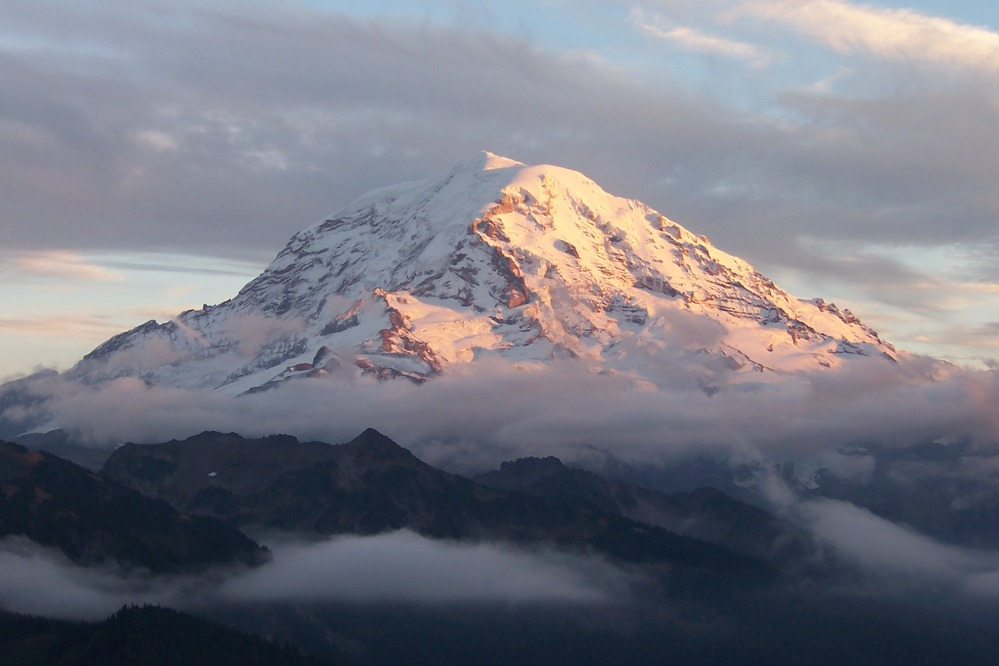
\includegraphics[keepaspectratio]{index_files/mediabag/hires-.jpg}}

}

\caption{\label{fig-rainier}Mount Rainier, also known by the Indigenous
name Tahoma, is an active volcano and 14,411 feet tall. Mount Rainier
National Park, which is 60 miles south-east of Seattle, Washington, was
founded in 1899. Photo credit:
\href{https://www.nps.gov/media/photo/gallery-item.htm?pg=5003191&id=ca60fce5-155d-4519-3e7c-1200750746f6&gid=CA4C9908-155D-4519-3E19303DAEADE22C}{NPS
(public domain)}.}

\end{figure}%

While the National Parks were originally created to protect precious,
beautiful lands and to make them accessible to everyday people---a noble
goal---it is important to remember that many of these lands were taken,
sometimes forcibly, from Native American people who already owned,
lived, and worked on them (Spence 2000; Beauchamp 2020). Today, there
are still calls for the NPS to
\href{https://www.theatlantic.com/magazine/archive/2021/05/return-the-national-parks-to-the-tribes/618395/}{return
the lands of the National Parks to Indigenous people.}

In a similar vein, scholars have shown that early environmental
conservation movements---movements that helped to spur the development
of the National Parks---were troublingly intertwined with racism and
eugenics movements (Beauchamp 2020). These prejudiced origins, combined
with continuing forms of environmental racism (e.g., many parks are
located far from cities, with limited public transporation options and
limited community outreach), have contributed to the marginalization of
people of color and other minorities in the parks. Research has shown
that white people visit the parks more than other racial groups (Weber
and Sultana 2013; Alba et al. 2022; Floyd and Johnson 2002). So while
the National Parks are technically open to everyone, they are not
equally accessible to everyone in the same way. And these exclusions
shape the parks' visitation data even before it's counted.

So when and why did visit counting start at the U.S. National Parks?
Well, according to the NPS, the counting of park visits started
\href{https://www.nps.gov/subjects/socialscience/visitor-use-statistics.htm}{as
early as 1904} (more than 10 years before the National Park Service
itself was officially created). But at this time, and for the next 50
years or so, their data collection methods were mostly
\href{https://www.nps.gov/subjects/socialscience/visitor-use-statistics.htm}{informal,
inconsistent, and low-tech}.

But in 1965, the NPS started getting serious about counting visits. That
year, the U.S. Congress passed
\href{https://www.everycrsreport.com/reports/RL33531.html}{The Land and
Water Conservation Fund Act of 1965}. This act created a new source of
government money specifically dedicated to protecting natural resources
and expanding outdoor recreation infrastructure. Because the act
stipulated that the amount of money allocated to each area should be
\href{https://www.nps.gov/subjects/socialscience/statistics-history.htm}{``proportional
to visitor use,''} the NPS buckled down on counting visitor use. They
\href{https://www.nps.gov/subjects/socialscience/statistics-history.htm}{``developed
and institutionalized a formal system for collecting, compiling and
reporting visitor use data.''}

In 1979, the NPS comprehensively changed their counting procedure, and
\href{(https://www.nps.gov/subjects/socialscience/visitor-use-statistics-dashboard.htm)}{all
parks began tracking vistor use by month} (as opposed to year) across 11
different statistics. This is why the datasets featured here begin in
1979.\footnote{The NPS also offers
  \href{https://irma.nps.gov/Stats/SSRSReports/National\%20Reports/Query\%20Builder\%20for\%20Historic\%20Annual\%20Recreation\%20Visits\%20(1904\%20-\%201979)}{annual
  visitation information between 1904-1979}, but it is a separate, less
  consistent dataset.} \textbf{Note: We aggregated monthly counts into
yearly counts for the dataset featured in this essay. A dataset with
visit counts by month is available in
\href{?tab=explore-the-data}{``Explore the Data.''}}

\begin{Shaded}
\begin{Highlighting}[]
\CommentTok{\# Note on installation: https://statsandr.com/blog/an{-}efficient{-}way{-}to{-}install{-}and{-}load{-}r{-}packages/}

\CommentTok{\# Load the dplyr package for data manipulation}
\CommentTok{\# Load the ggplot2 package for data visualization}
\CommentTok{\# Load "ggthemes", which let\textquotesingle{}s us use colorblind{-}compatible palettes. When we\textquotesingle{}ve only got one line, this will just be black.}
\CommentTok{\# Load "scales" for abbreviating axis labels}
\FunctionTok{library}\NormalTok{(dplyr, }\AttributeTok{warn =} \ConstantTok{FALSE}\NormalTok{)}
\FunctionTok{library}\NormalTok{(ggplot2)}
\FunctionTok{library}\NormalTok{(ggthemes)}
\FunctionTok{library}\NormalTok{(}\StringTok{"scales"}\NormalTok{)}

\CommentTok{\# Load National Park Visitation data}
\NormalTok{np\_data }\OtherTok{\textless{}{-}} \FunctionTok{read.csv}\NormalTok{(}\StringTok{"https://raw.githubusercontent.com/melaniewalsh/responsible{-}datasets{-}in{-}context/main/datasets/national{-}parks/US{-}National{-}Parks\_RecreationVisits\_1979{-}2023.csv"}\NormalTok{, }\AttributeTok{stringsAsFactors =} \ConstantTok{FALSE}\NormalTok{)}

\CommentTok{\# Specify the colorblind palette}
\NormalTok{cb\_palette }\OtherTok{\textless{}{-}} \FunctionTok{colorblind\_pal}\NormalTok{()(}\DecValTok{8}\NormalTok{)}

\CommentTok{\# Turn off scientific notation}
\FunctionTok{options}\NormalTok{(}\AttributeTok{scipen =} \DecValTok{999}\NormalTok{)}

\CommentTok{\# Filter down to Yellowstone National Park}
\NormalTok{yellowstone\_data }\OtherTok{\textless{}{-}}\NormalTok{ np\_data }\SpecialCharTok{\%\textgreater{}\%} \FunctionTok{filter}\NormalTok{(ParkName }\SpecialCharTok{==} \StringTok{"Yellowstone NP"}\NormalTok{)}

\CommentTok{\# Visualise it}
\FunctionTok{ggplot}\NormalTok{(}\AttributeTok{data =}\NormalTok{ yellowstone\_data) }\SpecialCharTok{+} 
  \FunctionTok{geom\_line}\NormalTok{(}\FunctionTok{aes}\NormalTok{(}\AttributeTok{x =}\NormalTok{ Year, }\AttributeTok{y =}\NormalTok{ RecreationVisits), }\AttributeTok{color =}\NormalTok{ cb\_palette[}\DecValTok{1}\NormalTok{]) }\SpecialCharTok{+} 
  \FunctionTok{labs}\NormalTok{(}\AttributeTok{title =} \StringTok{"Yellowstone National Park Visits (1979 {-} Present)"}\NormalTok{) }\SpecialCharTok{+}
  \CommentTok{\# abbreviate numbers by millions and thousands}
  \FunctionTok{scale\_y\_continuous}\NormalTok{(}\AttributeTok{labels =} \FunctionTok{label\_number}\NormalTok{(}\AttributeTok{scale\_cut =} \FunctionTok{cut\_short\_scale}\NormalTok{()))}
\end{Highlighting}
\end{Shaded}

\pandocbounded{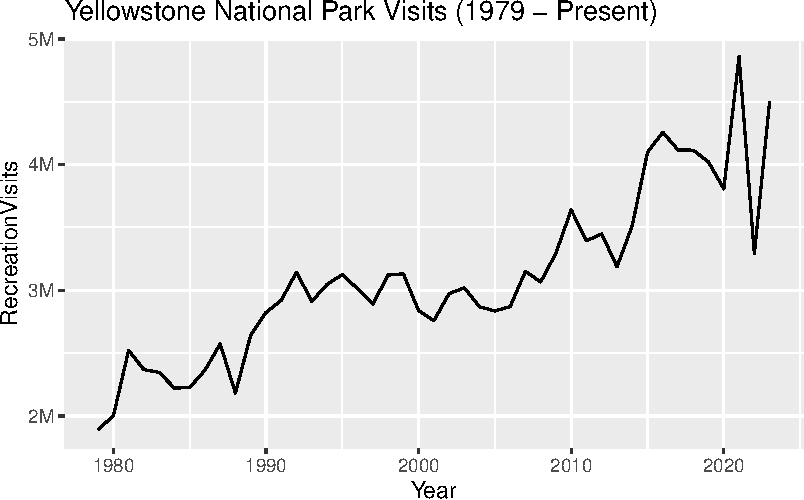
\includegraphics[keepaspectratio]{index_files/figure-pdf/unnamed-chunk-7-1.pdf}}

While today's National Park data collection system is more formal and
sophisticated than the one that the NPS used in 1904, there are still
many inconsistencies, flaws, and limitations (as the NPS
\href{https://www.nps.gov/subjects/socialscience/visitor-use-statistics-dashboard.htm}{openly
acknowledges}). This data does \emph{not} represent the \emph{exact}
number of people who visited the parks in the last 50 years---hardly!
Think about how difficult it would be to count every single one of the
millions of people who walked, hiked, backpacked, drove, shuttled,
canoed, biked, or skied into each of the 63 different parks since 1979.
These parks are located in dozens of different geographic areas,
including mountains, volcanoes, deserts, canyons, wetlands, forests, and
islands; the parks have experienced countless different weather
conditions during this time, including blizzards, hurricanes, wildfires,
avalanches, and extreme heat; and the parks have also been allocated
varying amounts of money and staff members to do the counting. Given all
this variability, it is simply not possible to count every single visit
to every single National Park ever.

We believe the National Park visit data is useful to study and consider
precisely for this reason: because it helps demonstrate that
\textbf{data never reflects reality precisely}. It also demonstrates
that collecting and analyzing data, even when it is flawed and
approximate, is sometimes worthwhile---but only if you fully understand
the data's flaws, limitations, and history, and only if you incorporate
these considerations into all subsequent analyses, interpretations, and
takeaways.

\subsection{Where did the data come from? Who collected
it?}\label{where-did-the-data-come-from-who-collected-it}

The National Park data on this website was originally organized and
published by the
\href{https://www.nps.gov/subjects/socialscience/visitor-use-statistics.htm}{NPS
Social Science Program}, which in turn runs the NPS Visitor Use
Statistics program, an initiative that coordinates visitor use
statistics across the parks. Thousands of staff members across all 63
parks were also involved in the data collection process.

According
\href{https://www.nps.gov/subjects/socialscience/statistics-history.htm}{to
the NPS}, the Visitor Use Statistics program aims to:

\begin{quote}
\begin{itemize}
\tightlist
\item
  Provide a statistically valid, reliable, and uniform method of
  collecting and reporting visitor use data for each independent unit
  administered by the NPS
\item
  Support regular collection, and timely publication, analysis and
  interpretation of these data
\item
  Enact quality control checks, verify measurements, and ensure
  consistency and comparability of data among areas of the NPS
\end{itemize}
\end{quote}

We accessed the original data through the NPS's
\href{https://irma.nps.gov/Stats/}{Visitor Use Statistics data portal},
which publishes visit use data in alignment with the program's stated
goals. Through this portal, anyone can generate reports and download
data for \href{https://irma.nps.gov/Stats/Reports/National}{different
visit use categories} and time periods---at both national and individual
park levels.

To download the data included here, we first selected
\href{https://irma.nps.gov/Stats/Reports/National}{``National Reports''}
in the data portal, and we then selected the
\href{https://irma.nps.gov/Stats/SSRSReports/National\%20Reports/Query\%20Builder\%20for\%20Public\%20Use\%20Statistics\%20(1979\%20-\%20Last\%20Calendar\%20Year)}{``Query
Builder for Public Use Statistics (1979 - Last Calendar Year)''} report
type. Here are the selections we made:

\begin{itemize}
\tightlist
\item
  For ``Park Types,'' we selected only ``National Parks.''
\item
  For ``Years,'' we selected all possible years (1979-2023).
\item
  For ``Regions,'' we selected all possible regions.
\item
  For ``Field Type,'' we selected only ``Recreation Visits'' (excluding
  the other 10 possible statistics: ``NonRecreation Visits,''
  ``Recreation Hours,'' ``NonRecreation Hours,'' ``Concessioner
  Lodging,'' ``Concessioner Camping,'' ``Tent Campers,'' ``RV Campers,''
  ``Backcountry Campers,'' ``NonRecreation Overnight Stays,'' and
  ``Miscellaneous Overnight Stays'').
\item
  For ``Additional Fields,'' we selected ``State'' and ``Region.''
\item
  We also selected the option of viewing the report as an annual summary
  of visit counts (as opposed to monthly visit counts).
\end{itemize}

\begin{figure}

\centering{

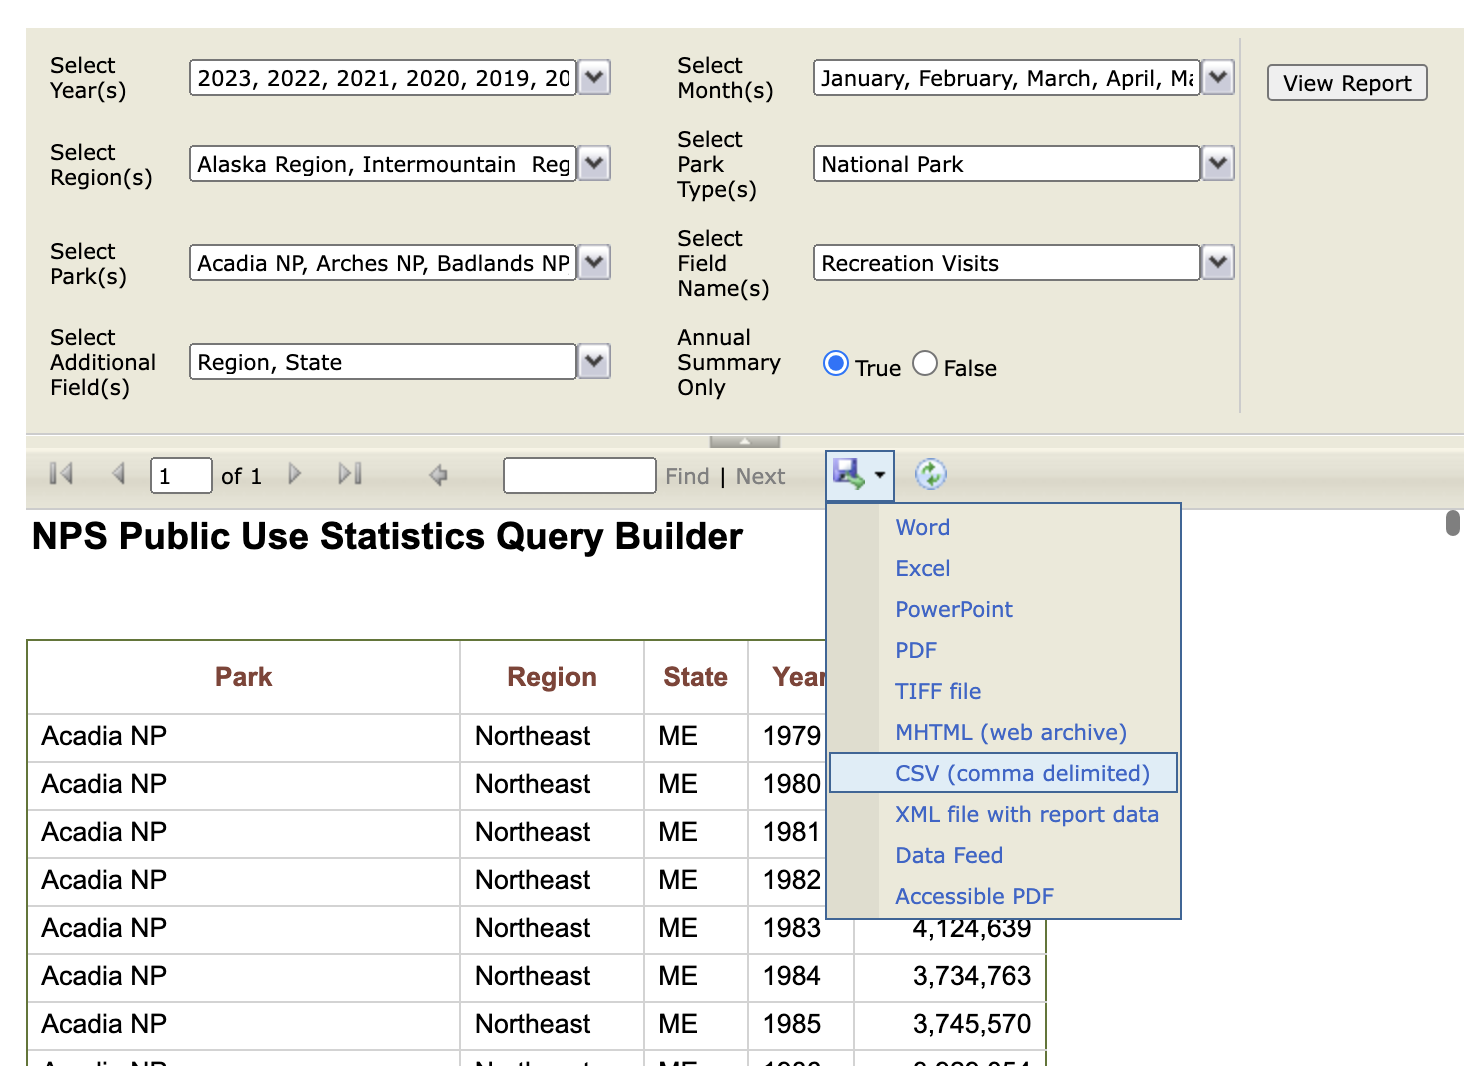
\includegraphics[width=0.9\linewidth,height=\textheight,keepaspectratio]{images/query-builder-csv-screenshot.png}

}

\caption{\label{fig-query-builder}Selections for National Park visit
data generated with
\href{https://irma.nps.gov/Stats/SSRSReports/National\%20Reports/Query\%20Builder\%20for\%20Public\%20Use\%20Statistics\%20(1979\%20-\%20Last\%20Calendar\%20Year)}{``Query
Builder for Public Use Statistics (1979 - Last Calendar Year)''}.}

\end{figure}%

If you choose to download this report as a CSV file, it will
unfortunately not look exactly like the report pictured in
Figure~\ref{fig-query-builder}; instead, the CSV will include all visit
and use types, and it will include visit and use information by month
rather than by year. When I (Melanie Walsh) have compiled this data to
share with my students in the past, I have sometimes downloaded the CSV
file, removed the columns that I'm not interested in, and aggregated the
data by year programatically. In other cases, I have simply copied and
pasted the annual summary report into a CSV file.

In either case, it is usually necessary to explicitly transform the
format of the ``RecreationVisits'' column into a number and to remove
the commas that separate the numbers by thousands (a transformation that
you can do with spreadsheet applications like Excel or Google Sheets, or
with a programming language like Python or R). Finally, we published the
data to this project's GitHub repository for easier storage and access.

\subsection{Why was the data collected? How is the data
used?}\label{why-was-the-data-collected-how-is-the-data-used}

The NPS collects visit data partly because the government requires it,
as we've already discussed. But the NPS also uses the visit data for
other internal purposes---to help determine which parks might need more
staff members and programming, which hiking trails might need more
maintenance, which natural areas might need more protection, or which
visitor centers might need more bathrooms.

The visit data also helps the communities and businesses surrounding the
parks understand how they can best provide and share resources, like
emergency vehicles, sanitation, and water. For example, if there's been
a large influx of hikers to Mount Rainier National Park in recent years,
that would be an important thing for the surrounding community to know.
Because those hikers would probably need more ambulance trips and rescue
helicopters (unfortunately but inevitably), and the surrounding towns
wouldn't want visitors to the National Park booking up all the available
emergency vehicles in town.

\begin{figure}

\centering{

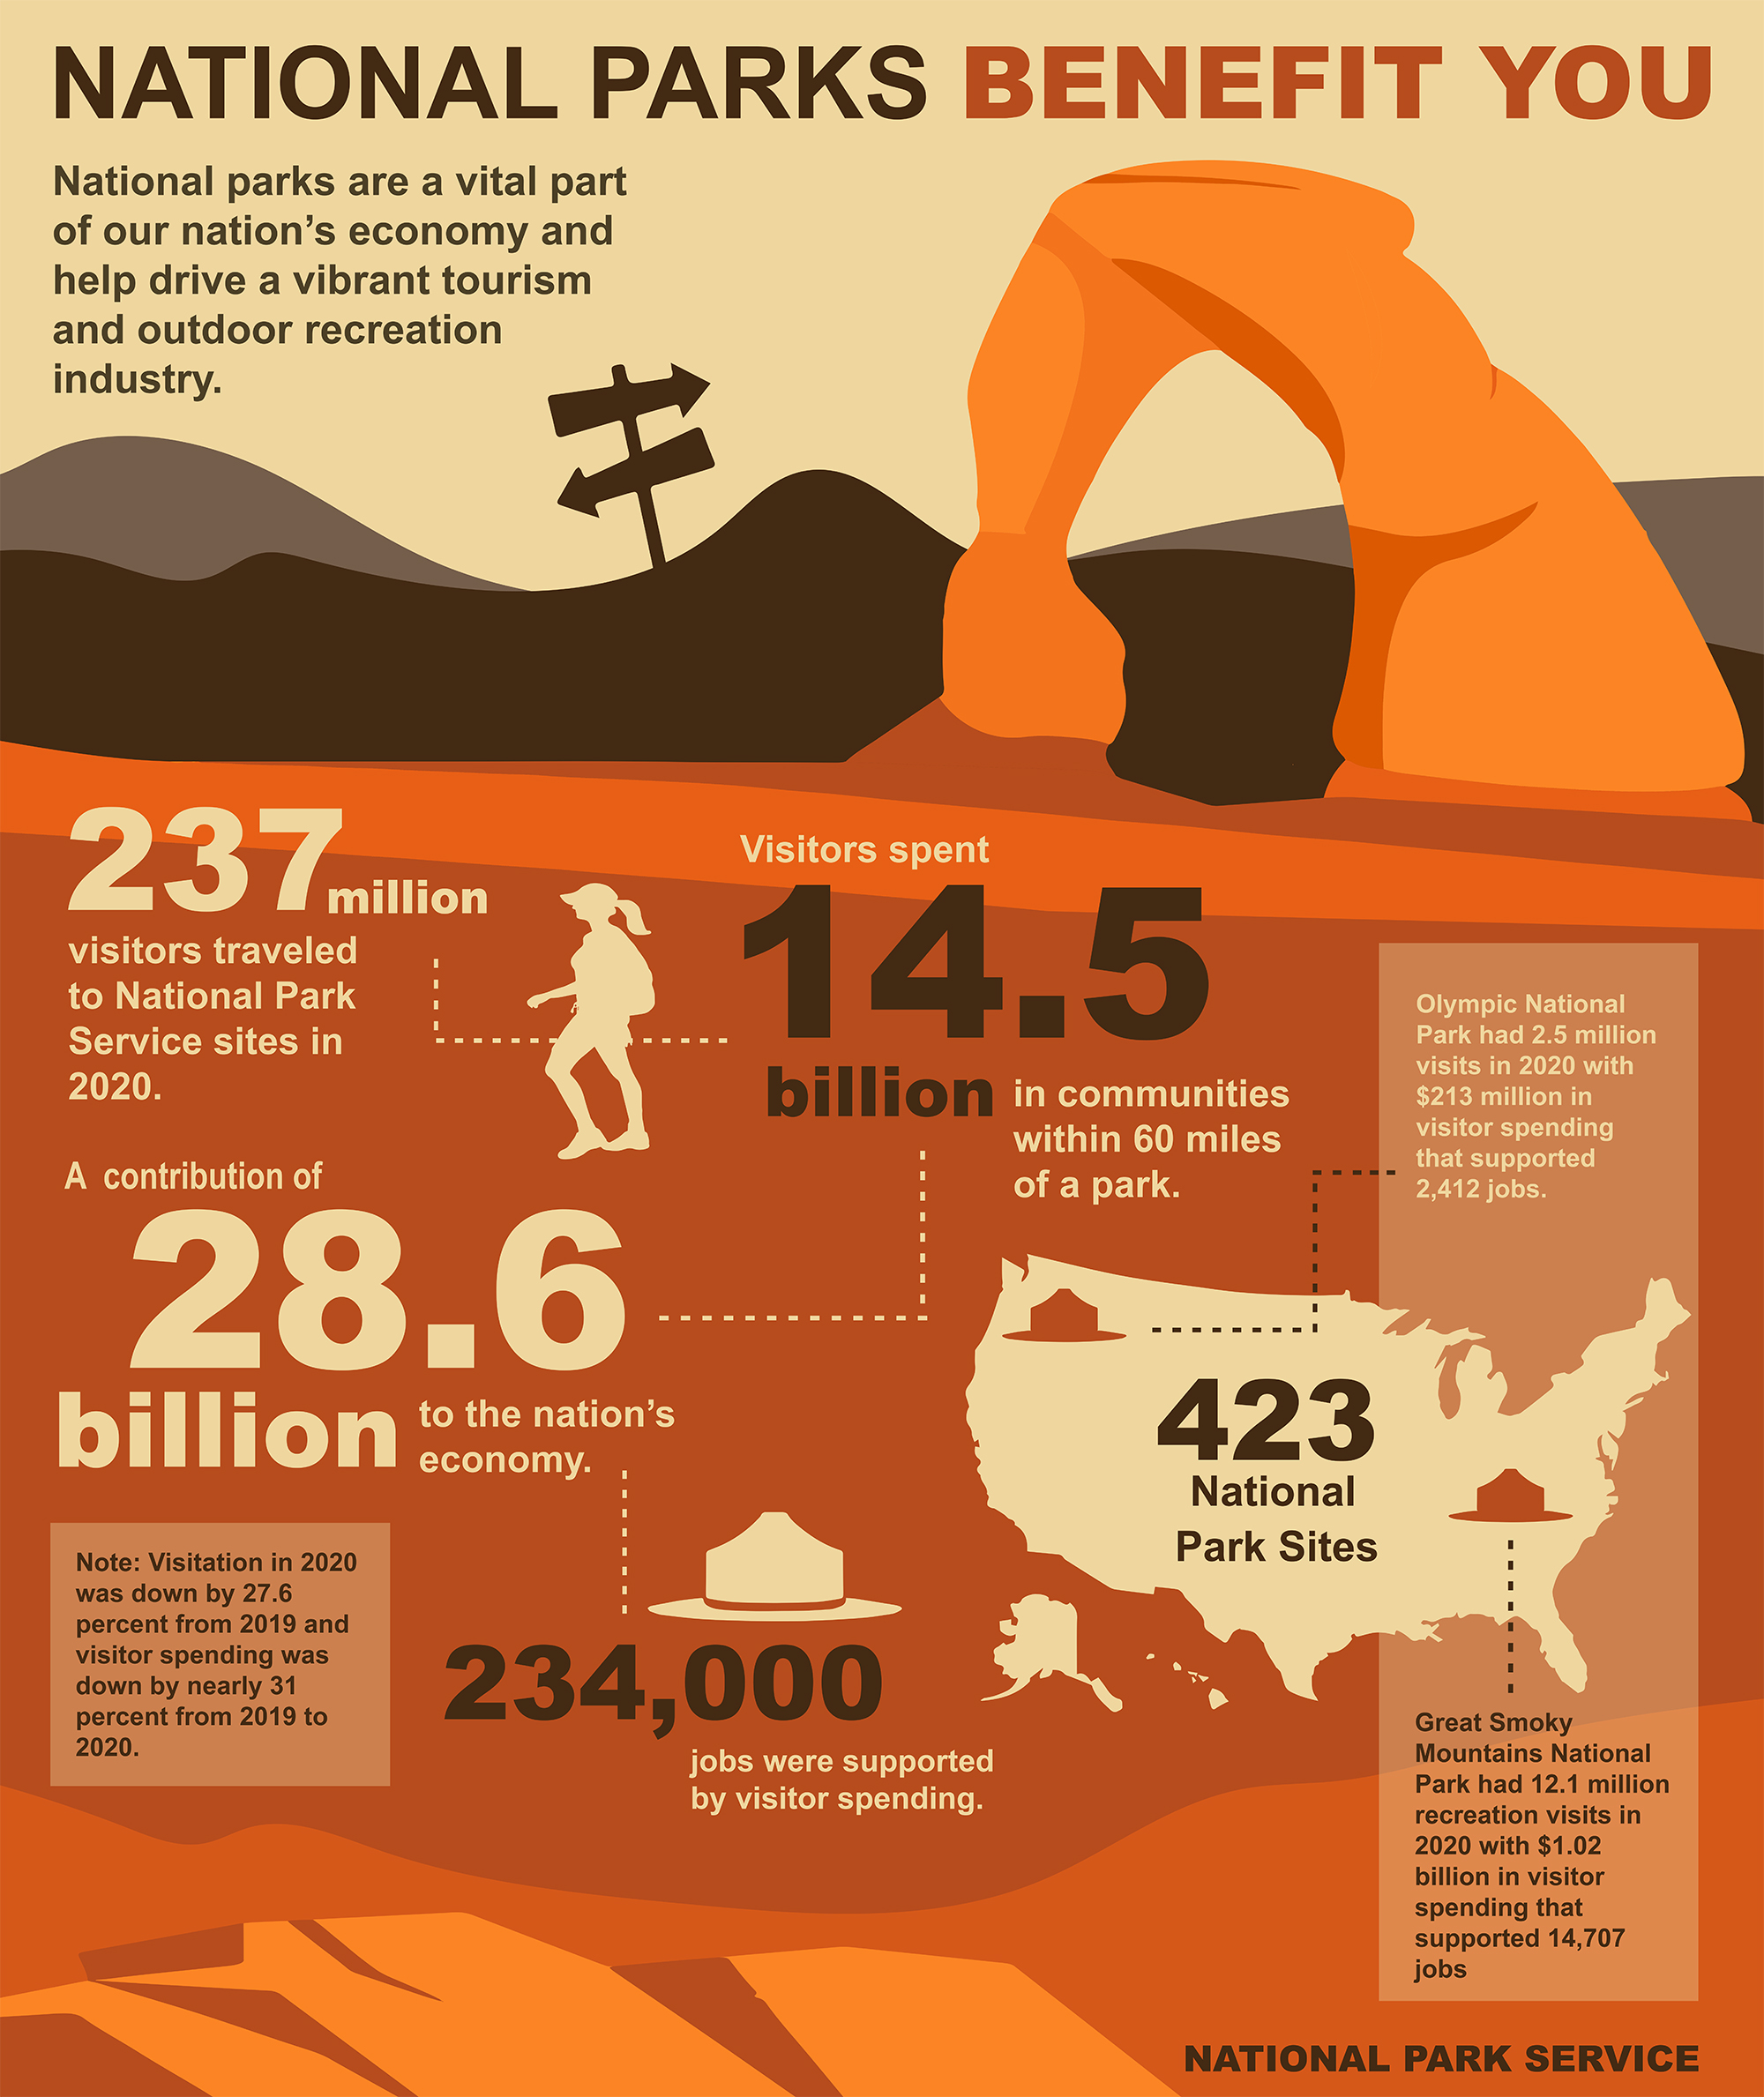
\includegraphics[width=0.9\linewidth,height=\textheight,keepaspectratio]{index_files/mediabag/ECONOMIC-2020.jpg}

}

\caption{\label{fig-economic-benefit}2021 report on NPS economic impact.
Graphic credit: \href{https://www.nps.gov/orgs/1207/vse2020.htm}{NPS}.}

\end{figure}%

The visitation data also helps the NPS estimate the beneficial
impact---economic and otherwise---that the parks have on nearby
communities and the nation at large (Figure~\ref{fig-economic-benefit}).
For example, in 2021, an
\href{https://www.nps.gov/grca/learn/news/visitor-use-spending-to-grand-canyon-2021.htm}{NPS
report} showed that ``4.5 million visitors to Grand Canyon National
Park\ldots spent an estimated \$710 million in gateway regions near the
park,'' which ``supported 9,390 jobs in the local area.'' These
estimations are important because they help the parks advocate for more
funding, support, and attention.

The data is also frequently reported on by journalists, who use it to
highlight the most popular parks and noteworthy visitation records, and
to point their readers to parks where they might be able to find some
peace and quiet (see articles in
\href{https://www.thrillist.com/news/nation/most-visited-national-parks-ranked-nps}{Thrillist},
\href{https://www.smithsonianmag.com/smart-news/most-and-least-popular-national-parks-2023-180983850/}{Smithsonian},
and
\href{https://www.cnn.com/travel/article/most-visited-us-national-park-sites-2022/index.html}{CNN}).

\begin{tcolorbox}[enhanced jigsaw, title=\textcolor{quarto-callout-tip-color}{\faLightbulb}\hspace{0.5em}{Discussion Question 1}, opacityback=0, bottomtitle=1mm, left=2mm, coltitle=black, opacitybacktitle=0.6, breakable, arc=.35mm, colframe=quarto-callout-tip-color-frame, toprule=.15mm, rightrule=.15mm, colback=white, colbacktitle=quarto-callout-tip-color!10!white, leftrule=.75mm, toptitle=1mm, titlerule=0mm, bottomrule=.15mm]

How else might the National Park visit data be used? How might it be
used by artists, historians, literary scholars, sociologists, or
librarians?

For more, see
\href{?tab=discussion-\%26-activities\#discussion-1}{Discussion Q 1}.

\end{tcolorbox}

\subsection{What's in the data? What ``counts'' as a
visit?}\label{whats-in-the-data-what-counts-as-a-visit}

Now that we know how the data is used, let's dive into the data itself.
What's actually in this dataset? What ``counts'' as a visit?

To get started, let's load the dataset and examine a random sample of
rows.

\begin{Shaded}
\begin{Highlighting}[]
\CommentTok{\# https://statsandr.com/blog/an{-}efficient{-}way{-}to{-}install{-}and{-}load{-}r{-}packages/}

\CommentTok{\# Load the dplyr package}
\FunctionTok{library}\NormalTok{(dplyr, }\AttributeTok{warn =} \ConstantTok{FALSE}\NormalTok{)}

\CommentTok{\# Load National Park Visitation data}
\NormalTok{np\_data }\OtherTok{\textless{}{-}} \FunctionTok{read.csv}\NormalTok{(}\StringTok{"https://raw.githubusercontent.com/melaniewalsh/responsible{-}datasets{-}in{-}context/main/datasets/national{-}parks/US{-}National{-}Parks\_RecreationVisits\_1979{-}2023.csv"}\NormalTok{, }\AttributeTok{stringsAsFactors =} \ConstantTok{FALSE}\NormalTok{)}

\DocumentationTok{\#\# Look at the structure of the dataset, randomly sample 10 rows}
\NormalTok{np\_data }\SpecialCharTok{\%\textgreater{}\%} \FunctionTok{slice\_sample}\NormalTok{(}\AttributeTok{n =} \DecValTok{10}\NormalTok{)}
\end{Highlighting}
\end{Shaded}

\begin{longtable}[]{@{}
  >{\raggedright\arraybackslash}p{(\linewidth - 8\tabcolsep) * \real{0.4324}}
  >{\raggedright\arraybackslash}p{(\linewidth - 8\tabcolsep) * \real{0.1892}}
  >{\raggedright\arraybackslash}p{(\linewidth - 8\tabcolsep) * \real{0.0811}}
  >{\raggedleft\arraybackslash}p{(\linewidth - 8\tabcolsep) * \real{0.0676}}
  >{\raggedleft\arraybackslash}p{(\linewidth - 8\tabcolsep) * \real{0.2297}}@{}}
\toprule\noalign{}
\begin{minipage}[b]{\linewidth}\raggedright
ParkName
\end{minipage} & \begin{minipage}[b]{\linewidth}\raggedright
Region
\end{minipage} & \begin{minipage}[b]{\linewidth}\raggedright
State
\end{minipage} & \begin{minipage}[b]{\linewidth}\raggedleft
Year
\end{minipage} & \begin{minipage}[b]{\linewidth}\raggedleft
RecreationVisits
\end{minipage} \\
\midrule\noalign{}
\endhead
\bottomrule\noalign{}
\endlastfoot
Petrified Forest NP & Intermountain & AZ & 2009 & 631613 \\
Carlsbad Caverns NP & Intermountain & NM & 1991 & 679450 \\
Arches NP & Intermountain & UT & 1992 & 799831 \\
Carlsbad Caverns NP & Intermountain & NM & 2016 & 466773 \\
White Sands NP & Intermountain & NM & 1987 & 567613 \\
Black Canyon of the Gunnison NP & Intermountain & CO & 1985 & 266012 \\
Glacier Bay NP \& PRES & Alaska & AK & 2008 & 418911 \\
North Cascades NP & Pacific West & WA & 1990 & 456444 \\
Big Bend NP & Intermountain & TX & 2019 & 463832 \\
Mammoth Cave NP & Southeast & KY & 2001 & 1883580 \\
\end{longtable}

Here we see five columns -- ``ParkName'', ``Region'', ``State'',
``Year'', and ``RecreationVisits.'' The first four are pretty
self-explanatory, but why is the fifth labelled ``RecreationVisits''
rather than ``Visits'' or ``Visitors''?

It turns out that the NPS counts visits, not visitors (which would be
more difficult to track), and they distinguish between different
\emph{kinds} of visits to their parks. First, there are
\emph{reportable} and \emph{non-reportable} visits. When NPS employees
or their families go to the parks, these visits are
\emph{non-reportable}. But pretty much everything else is
\emph{reportable}. Within \emph{reportable} visits, there are two more
types of visits: \emph{recreation} and \emph{non-recreation} visits.
Recreation visits are when people are visiting the parks for fun,
vacation, exercise, school trips, etc., and non-recreation visits are
when people are visiting the parks for other reasons. For example, some
people need to travel \emph{through} the parks, either because a highway
runs through the park, or because they live on ``inholdings'' (private
property that is surrounded by a National Park on all sides). Other
people need to visit the parks because they have business to conduct.

Here's a
\href{https://www.nps.gov/subjects/socialscience/nps-visitor-use-statistics-definitions.htm}{full
list of the ``reportable non-recreation'' visits}, according to the NPS:

\begin{quote}
\begin{itemize}
\tightlist
\item
  Persons going to and from inholdings across significant parts of park
  land;
\item
  Commuter and other traffic using NPS-administered roads or waterways
  through a park for their convenience;
\item
  Trades-people with business in the park;
\item
  Any civilian activity a part of or incidental to the pursuit of a
  gainful occupation (e.g., guides);
\item
  Government personnel (other than NPS employees) with business in the
  park;
\item
  Citizens using NPS buildings for civic or local government business,
  or attending public hearings;
\item
  Outside research activities (visits and overnights) if independent of
  NPS legislated interests (e.g.~meteorological research).
\end{itemize}
\end{quote}

Carefully reviewing this list reveals that the term ``recreation visit''
excludes a significant number of visits and individuals. It also raises
important questions about how the NPS distinguishes between different
types of visits, which we will explore further below.

\begin{tcolorbox}[enhanced jigsaw, title=\textcolor{quarto-callout-tip-color}{\faLightbulb}\hspace{0.5em}{Discussion Question 2}, opacityback=0, bottomtitle=1mm, left=2mm, coltitle=black, opacitybacktitle=0.6, breakable, arc=.35mm, colframe=quarto-callout-tip-color-frame, toprule=.15mm, rightrule=.15mm, colback=white, colbacktitle=quarto-callout-tip-color!10!white, leftrule=.75mm, toptitle=1mm, titlerule=0mm, bottomrule=.15mm]

What are the potential consequences of considering these visits to be
\emph{non-recreation} vs.~\emph{recreation} visits?

For more, see
\href{?tab=discussion-\%26-activities\#discussion-2}{Discussion Q 2}.

\end{tcolorbox}

\begin{figure}

\centering{

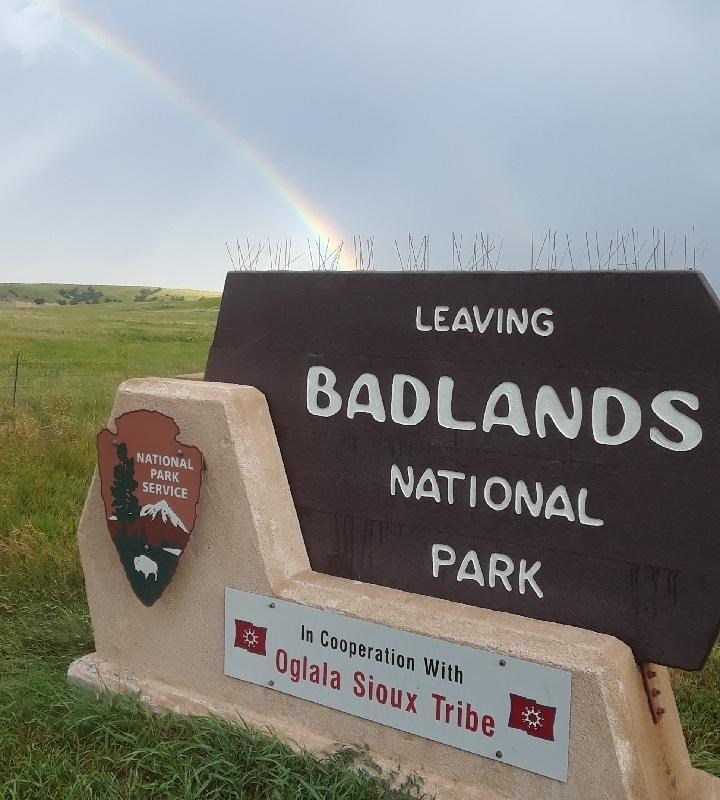
\includegraphics[width=0.8\linewidth,height=\textheight,keepaspectratio]{index_files/mediabag/62A55536-BD00-F301-4.jpg}

}

\caption{\label{fig-badlands}Badlands National Park sign, gesturing to
the South Unit's co-management between the Oglala Sioux Tribe and the
NPS. Photo credit:
\href{https://www.nps.gov/common/uploads/structured_data/62A55536-BD00-F301-462744BEDD8BA664.jpg?width=800&height=800&mode=crop&quality=90}{NPS}.}

\end{figure}%

The list also prompts us to consider those whose presence in the parks
doesn't fit neatly into the ``visit'' category at all. For instance, a
portion of Badlands National Park in South Dakota overlaps with the Pine
Ridge Indian Reservation, which is
\href{https://www.nps.gov/articles/000/stronghold-district.htm}{``owned
by the Oglala Sioux Tribe and managed by the National Park Service under
an agreement with the Tribe.''} According to the NPS, when traveling
through this area, visitors might encounter ``signs of religious
worship'' from Tribal members, such as ``prayer sticks'' or pieces of
``brightly colored fabric tied to a shrub,'' and they are advised to
``respect {[}the Tribal members'{]} beliefs and practices and leave
these objects.'' These symbols woven into the landscape underscore that
members of the Oglala Sioux Tribe are not visitors to the Badlands but
stewards and residents with deep ancestral connections. It reveals that
the National Park data's focus on ``visits''-----whether reportable or
non-reportable, recreational or non-recreational-----fails to account
for those who are not visitors, those who own and live on the land, and
those whose ancestors lived on the land before the NPS even existed.

\subsection{How was the data
collected?}\label{how-was-the-data-collected}

At this point, we know \emph{what} counts as visit, but \emph{how} does
the NPS actually count these visits and collect data? And how do they
differentiate between the different types of visits? Take a moment and
see if you come up with a few guesses.

It turns out that each park counts visits differently. At many parks,
\emph{each entrance} at each park even counts visits differently.

If you go to the \href{https://irma.nps.gov/Stats/Reports/Park}{``Park
Reports''} tab in the NPS Data Portal, you can look up an individual
park and download a PDF file called ``Visitor Use Counting Procedures,''
which details exactly what procedures they use to count visits at this
park. Most of the parks have several PDFs because their counting
procedures have changed many times over the years!

\begin{tcolorbox}[enhanced jigsaw, title=\textcolor{quarto-callout-tip-color}{\faLightbulb}\hspace{0.5em}{Activity 2}, opacityback=0, bottomtitle=1mm, left=2mm, coltitle=black, opacitybacktitle=0.6, breakable, arc=.35mm, colframe=quarto-callout-tip-color-frame, toprule=.15mm, rightrule=.15mm, colback=white, colbacktitle=quarto-callout-tip-color!10!white, leftrule=.75mm, toptitle=1mm, titlerule=0mm, bottomrule=.15mm]

How are the procedures for three different parks similar or different?
For more, see
\href{?tab=discussion-\%26-activities\#activity-2}{Activity 2}.

\end{tcolorbox}

\begin{figure}

\centering{

\includegraphics[width=3.125in,height=\textheight,keepaspectratio]{index_files/mediabag/Metrocount_vehicle_c.jpg-20110223182337}

}

\caption{\label{fig-pneumatic-tube}An example of a pneumatic tube
traffic counter, installed above the road.}

\end{figure}%

To count visits, most parks use a combination of automatic traffic
counters and manual counting-----that is, staff members who use their
eyeballs to literally count the number of people arriving by foot, bike,
bus, cross-country skis, snowmobile, boat, canoe, etc.

Whether automatic or manual, these counts are usually modified with
specially designed mathematical formulas, which are supposed to produce
the most accurate estimate for recreation visits at any given location.
Staff members add, subtract, multiply, and divide the counts based on a
variety of factors, such as the season or the entrance (e.g.~assuming
that more people would likely be arriving in a car in the summer months
at the most popular gate than in the winter months at the least popular
gate).

\begin{figure}[H]

{\centering \pandocbounded{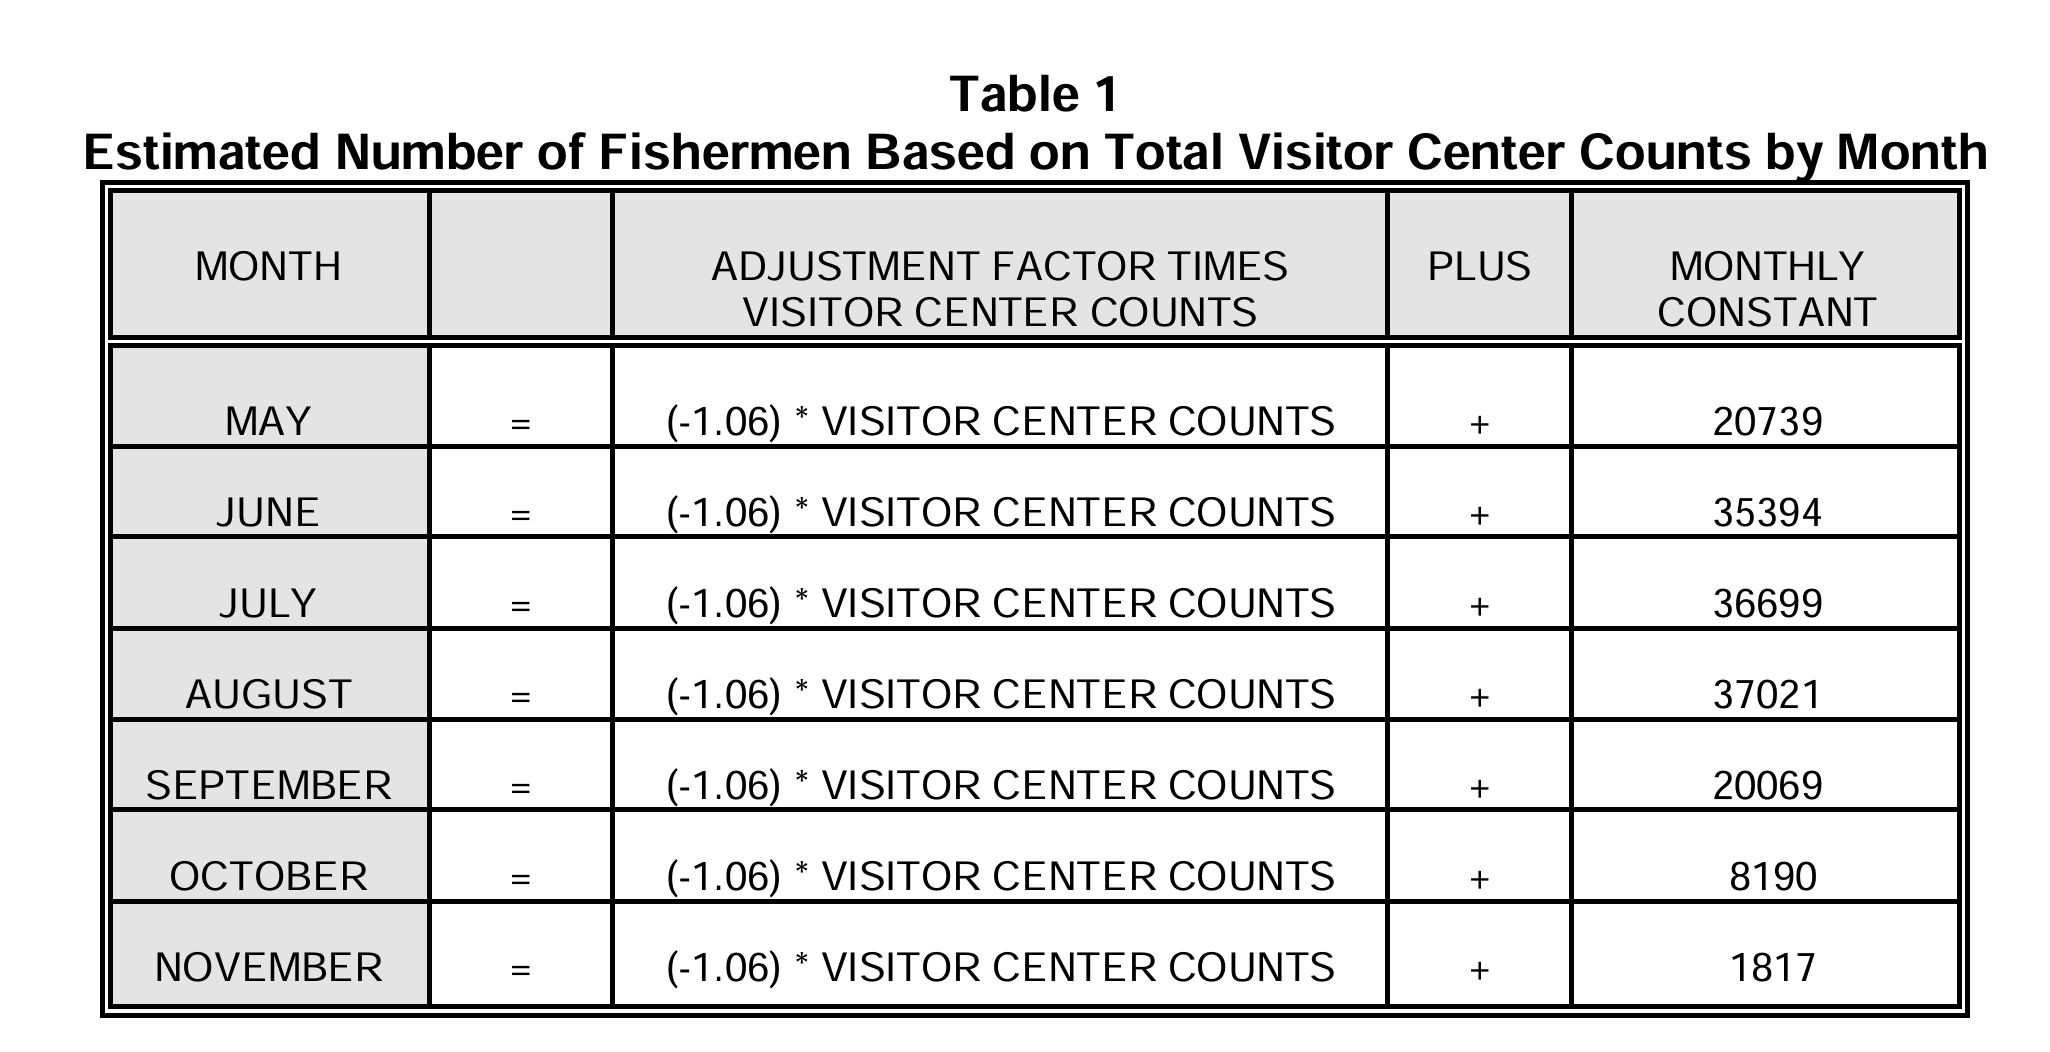
\includegraphics[keepaspectratio]{images/Voyageurs-table1.png}}

}

\caption{Table 1 from ``VOYAGEURS NATIONAL PARK PUBLIC USE REPORTING AND
COUNTING INSTRUCTIONS.'' Find the document here:
https://irma.nps.gov/Stats/Reports/Park.}

\end{figure}%

For instance, in the summer months (May through November) at Voyageurs
National Park in northern Minnesota---a park dominated by lakes and
waterways---they \href{https://irma.nps.gov/Stats/Reports/Park}{estimate
visits} by taking the number of visits to visitor centers, and then
adding the estimated number of fishermen, houseboaters, and backcountry
overnight stays. To take just one of these categories as an example,
they estimate the number of fishermen by ``taking the sum of the visitor
center counts and applying the regression equation in Table 1,'' which
is displayed above. In August, that number would be
\texttt{(-1.06)\ *\ VISITOR\ CENTER\ COUNTS\ \ +\ \ 37,021}. However, if
the month is November, and if the visitor count exceeds 17,00, ``then
fishermen are estimated at 0.'' These detailed instructions point to the
countless decisions and methodological choices that underlie the
National Park visit data. These manipulations are arguably necessary to
achieve ``statistically valid, reliable, and uniform'' collection
methods and data, as is the program's goal, but they also reveal the
ever persistent gap between recorded data and reality.

\begin{Shaded}
\begin{Highlighting}[]
\CommentTok{\# Filter down to Voyageurs National Park}
\NormalTok{voyageurs\_data }\OtherTok{\textless{}{-}}\NormalTok{ np\_data }\SpecialCharTok{\%\textgreater{}\%} \FunctionTok{filter}\NormalTok{(ParkName }\SpecialCharTok{==} \StringTok{"Voyageurs NP"}\NormalTok{)}

\CommentTok{\# Visualizee it}
\FunctionTok{ggplot}\NormalTok{(}\AttributeTok{data =}\NormalTok{ voyageurs\_data) }\SpecialCharTok{+} 
  \FunctionTok{geom\_line}\NormalTok{(}\FunctionTok{aes}\NormalTok{(}\AttributeTok{x =}\NormalTok{ Year, }\AttributeTok{y =}\NormalTok{ RecreationVisits), }\AttributeTok{color =}\NormalTok{ cb\_palette[}\DecValTok{8}\NormalTok{]) }\SpecialCharTok{+} 
  \FunctionTok{labs}\NormalTok{(}\AttributeTok{title =} \StringTok{"Voyageurs National Park Visits (1979 {-} Present)"}\NormalTok{) }\SpecialCharTok{+}
  \CommentTok{\# abbreviate numbers by millions and thousands}
  \FunctionTok{scale\_y\_continuous}\NormalTok{(}\AttributeTok{labels =} \FunctionTok{label\_number}\NormalTok{(}\AttributeTok{scale\_cut =} \FunctionTok{cut\_short\_scale}\NormalTok{()))}
\end{Highlighting}
\end{Shaded}

\pandocbounded{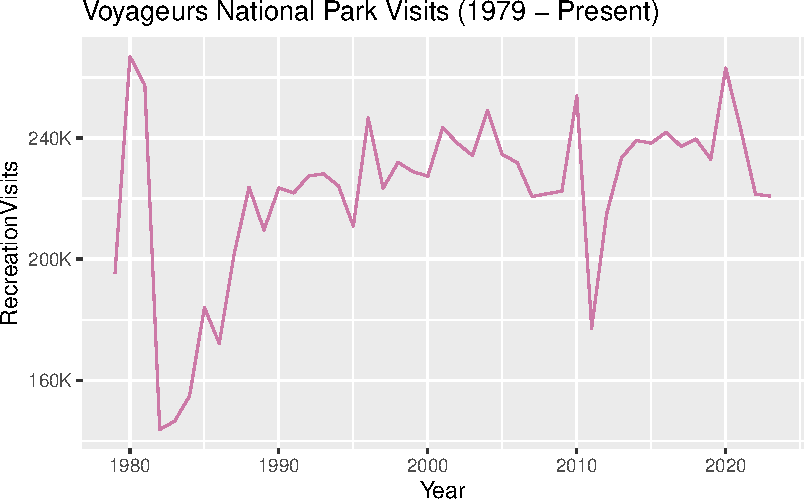
\includegraphics[keepaspectratio]{index_files/figure-pdf/unnamed-chunk-9-1.pdf}}

Consider, next, Everglades National Park in Florida. At the Shark Valley
Entrance, there is a pneumatic tube traffic counter
(Figure~\ref{fig-pneumatic-tube}) that counts the number of cars that
pass over it. The Everglades NP staff members then apply different
mathematical operations to this number in order to arrive at what they
think is the most accurate estimate of recreation visits:

\begin{quote}
The traffic count is divided by 2 to account for entry and exit. The
adjusted traffic count is reduced by the number of buses, the number of
bicycles counted when the entrance station is open, 127 bicycles per
month to account for after-hours use, and by 200 non-recreation vehicles
per month October through May and 100 non-recreation vehicles per month
June through September. The traffic count is further reduced by 350
non-reportable (NPS) vehicles per month. The reduced count is multiplied
by 2.17 persons per vehicle.
\end{quote}

Like Voyageurs NP in Minnesota, Everglades NP modifies their raw visit
data in many ways. Once again, these modifications are arguably
necessary, but they are nevertheless extensive and almost certainly
subject to debate.

What's more, the devices that the NPS uses to count visits---such as
pneumatic tube counters or induction loop counters (magnetized coils of
wire that are installed under a road, and that ``trip'' when a vehicle
passes over them)---sometimes \emph{break}.

\begin{figure}

\centering{

\includegraphics[width=3.125in,height=\textheight,keepaspectratio]{index_files/mediabag/Inductance_detectors.jpg}

}

\caption{\label{fig-induction}An example of an induction loop, installed
beneath a road (making it harder to detect when it breaks!).}

\end{figure}%

For example,
\href{https://irma.nps.gov/Stats/SSRSReports/Park\%20Specific\%20Reports/Monthly\%20Visitation\%20Comments\%20By\%20Park?Park=CRLA}{according
to the NPS data logs}, the induction loop counter at one of the main
entrances at Crater Lake National Park in Oregon broke in 2012 and
wasn't repaired for at least a year:

\begin{quote}
2/1/2012 \textbar{} The Traffic Counter at Annie Springs Entrance
Station was not functioning properly and therefore we have a count of
zero.
\end{quote}

\begin{quote}
3/1/2012 \textbar{} Broken counter at Annie Springs Entrance, unable to
record numbers.
\end{quote}

\begin{quote}
4/1/2012 \textbar{} Traffic counter was broken for the beginning of the
month and may have low numbers.
\end{quote}

\begin{quote}
10/1/2012 \textbar{} Counts estimated by Butch
\end{quote}

\begin{quote}
11/1/2012 \textbar{} TRAFFIC COUNT AT ANNIE SPRINGS ENTRANCE NOT
AVAILIBLE
\end{quote}

\begin{quote}
12/1/2012 \textbar{} TRAFFIC COUNT AT ANNIE SPRINGS ENTRANCE NOT
AVAILIBLE
\end{quote}

\begin{quote}
1/1/2013 \textbar{} Traffic count at Annie Springs estimated.
\end{quote}

\begin{quote}
2/1/2013 \textbar{} Traffic count at Annie Springs estimated.
\end{quote}

In some months, the broken counter meant that the number of recorded
visits at this entrace was recorded as zero. In other months, park
staff---including someone named Butch---decided to estimate the counts.

You can see a similar, but more severe, example of a broken counter at
Carlsbad Caverns National Park in California, where it appears that
visits have had a recent decline since 2019:

\begin{Shaded}
\begin{Highlighting}[]
\CommentTok{\# Load the "ggplot2" package (which we\textquotesingle{}ll be using a lot more)}
\FunctionTok{library}\NormalTok{(ggplot2)}

\CommentTok{\# Let\textquotesingle{}s also load "ggthemes", which let\textquotesingle{}s us use colorblind{-}compatible palettes. When we\textquotesingle{}ve only got one line, this will just be black.}
\FunctionTok{library}\NormalTok{(ggthemes)}

\CommentTok{\# And specify the colorblind palette}
\NormalTok{cb\_palette }\OtherTok{\textless{}{-}} \FunctionTok{colorblind\_pal}\NormalTok{()(}\DecValTok{8}\NormalTok{)}

\CommentTok{\# Turn off scientific notation}
\FunctionTok{options}\NormalTok{(}\AttributeTok{scipen =} \DecValTok{999}\NormalTok{)}

\CommentTok{\# Filter down to Carlsbad Caverns National Park}
\NormalTok{carlsbad\_data }\OtherTok{\textless{}{-}}\NormalTok{ np\_data }\SpecialCharTok{\%\textgreater{}\%} \FunctionTok{filter}\NormalTok{(ParkName }\SpecialCharTok{==} \StringTok{"Carlsbad Caverns NP"}\NormalTok{)}

\CommentTok{\# Visualise it}
\FunctionTok{ggplot}\NormalTok{(}\AttributeTok{data =}\NormalTok{ carlsbad\_data) }\SpecialCharTok{+} 
  \FunctionTok{geom\_line}\NormalTok{(}\FunctionTok{aes}\NormalTok{(}\AttributeTok{x =}\NormalTok{ Year, }\AttributeTok{y =}\NormalTok{ RecreationVisits), }\AttributeTok{color =}\NormalTok{ cb\_palette[}\DecValTok{2}\NormalTok{]) }\SpecialCharTok{+} 
  \FunctionTok{labs}\NormalTok{(}\AttributeTok{title =} \StringTok{"Carlsbad Caverns National Park Visits (1979 {-} Present)"}\NormalTok{) }\SpecialCharTok{+}
  \CommentTok{\# abbreviate numbers by millions and thousands}
  \FunctionTok{scale\_y\_continuous}\NormalTok{(}\AttributeTok{labels =} \FunctionTok{label\_number}\NormalTok{(}\AttributeTok{scale\_cut =} \FunctionTok{cut\_short\_scale}\NormalTok{()))}
\end{Highlighting}
\end{Shaded}

\pandocbounded{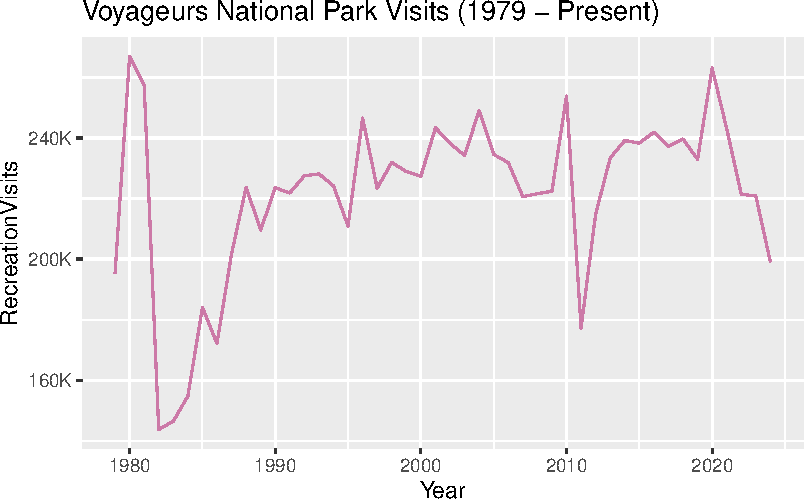
\includegraphics[keepaspectratio]{index_files/figure-pdf/unnamed-chunk-10-1.pdf}}

This decline may be due, in part, to the COVID-19 pandemic. But the NPS
logs also show that the main induction loop counter at Carlsbad Caverns
\href{https://irma.nps.gov/Stats/SSRSReports/Park\%20Specific\%20Reports/Monthly\%20Visitation\%20Comments\%20By\%20Park?Park=CAVE}{broke
in 2019 and has remained broken for multiple years}:

\begin{quote}
9/1/2019 \textbar{} Traffic counter apparently has been broken since
July. Traffic counts are estimated.
\end{quote}

\begin{quote}
4/1/2020 \textbar{} Main road traffic counter is broken, I have
estimated the count.
\end{quote}

\begin{quote}
12/1/2020 \textbar{} Corona virus closure that began in November ended
on December 4th. Main road traffic counter remains broken.Possible
problem with Loop Road counter.
\end{quote}

\begin{quote}
4/1/2022 Main road traffic counter remains broken. Rattlesnake Springs
traffic counter seems to be off, I will henceforth provide estimates.
\end{quote}

\begin{quote}
9/1/2023 \textbar{} Loop Road and backcountry closed due to flood
damage. Slaughter Canyon Cave remains closed Traffic counter on main
road remains broken.
\end{quote}

\begin{tcolorbox}[enhanced jigsaw, title=\textcolor{quarto-callout-tip-color}{\faLightbulb}\hspace{0.5em}{Activity 1}, opacityback=0, bottomtitle=1mm, left=2mm, coltitle=black, opacitybacktitle=0.6, breakable, arc=.35mm, colframe=quarto-callout-tip-color-frame, toprule=.15mm, rightrule=.15mm, colback=white, colbacktitle=quarto-callout-tip-color!10!white, leftrule=.75mm, toptitle=1mm, titlerule=0mm, bottomrule=.15mm]

Now that we've talked about how data is collected (and the fragility of
some of those methods), it's a good time to think about how even the
same method, deployed at different places, might be differently
unreliable. For more, see
\href{?tab=discussion-\%26-activities\#activity-1-1}{Activity 1}.

\end{tcolorbox}

\subsection{What data is missing? How is uncertainty
handled?}\label{what-data-is-missing-how-is-uncertainty-handled}

We already know that there is a lot missing from the National Park visit
data. There are people who never make it the parks---and thus never make
it into the dataset---because of environmental racism and a history of
discrimination and colonialism that is intertwined with the parks. There
are people who don't fit neatly into the category of a visit, such as
those who live inside the parks. There are also people who are missed by
the parks' various counting procedures and manipulations.

What else might be missing or uncertain? It turns out that the data
itself can point us to some answers. An important step in Exploratory
Data Analysis (EDA) is to analyze key summary statistics for your data,
such as maximum, minimum, or average values. This step can reveal
important patterns, problems, or inconsistencies in the data, and point
to parts of a dataset's backstory that need to be researched and
understood further. Exploring summary statistics for the National Park
data--- specifically, minimum values---reveals a few curious outliers
that point us to key areas of uncertainty.

If you filter the National Park visit data for the parks with the lest
(or minimum) number of visits since 1979, you will notice that there are
some parks that had \emph{zero} visits in a given year.

\begin{Shaded}
\begin{Highlighting}[]
\CommentTok{\# Filter for minimum RecVisits}
\NormalTok{least\_visited }\OtherTok{\textless{}{-}}\NormalTok{ np\_data }\SpecialCharTok{\%\textgreater{}\%} \FunctionTok{filter}\NormalTok{(RecreationVisits }\SpecialCharTok{==} \FunctionTok{min}\NormalTok{(RecreationVisits))}

\CommentTok{\# Number of rows for least visited}
\NormalTok{num\_rows }\OtherTok{\textless{}{-}} \FunctionTok{nrow}\NormalTok{(least\_visited)}

\CommentTok{\# Show some of them}
\NormalTok{least\_visited  }\SpecialCharTok{\%\textgreater{}\%} \FunctionTok{slice\_sample}\NormalTok{(}\AttributeTok{n =} \FunctionTok{min}\NormalTok{(}\DecValTok{10}\NormalTok{, num\_rows))}
\end{Highlighting}
\end{Shaded}

\begin{longtable}[]{@{}
  >{\raggedright\arraybackslash}p{(\linewidth - 8\tabcolsep) * \real{0.4384}}
  >{\raggedright\arraybackslash}p{(\linewidth - 8\tabcolsep) * \real{0.1781}}
  >{\raggedright\arraybackslash}p{(\linewidth - 8\tabcolsep) * \real{0.0822}}
  >{\raggedleft\arraybackslash}p{(\linewidth - 8\tabcolsep) * \real{0.0685}}
  >{\raggedleft\arraybackslash}p{(\linewidth - 8\tabcolsep) * \real{0.2329}}@{}}
\toprule\noalign{}
\begin{minipage}[b]{\linewidth}\raggedright
ParkName
\end{minipage} & \begin{minipage}[b]{\linewidth}\raggedright
Region
\end{minipage} & \begin{minipage}[b]{\linewidth}\raggedright
State
\end{minipage} & \begin{minipage}[b]{\linewidth}\raggedleft
Year
\end{minipage} & \begin{minipage}[b]{\linewidth}\raggedleft
RecreationVisits
\end{minipage} \\
\midrule\noalign{}
\endhead
\bottomrule\noalign{}
\endlastfoot
Katmai NP \& PRES & Alaska & AK & 1995 & 0 \\
Kobuk Valley NP & Alaska & AK & 2014 & 0 \\
National Park of American Samoa & Pacific West & AS & 2003 & 0 \\
Kobuk Valley NP & Alaska & AK & 2015 & 0 \\
\end{longtable}

You might guess that there are no visits in these years because these
parks are all located in remote places, like rural Alaska or American
Samoa.

If we look at the visitation trends for Kobuk Valley National Park in
Alaska, for example, we can see that a couple of years with zero visits
isn't a huge aberration from the trend:

\begin{Shaded}
\begin{Highlighting}[]
\CommentTok{\# Filter down to Mount Rainier National Park}
\NormalTok{kobuk\_data }\OtherTok{\textless{}{-}}\NormalTok{ np\_data }\SpecialCharTok{\%\textgreater{}\%} \FunctionTok{filter}\NormalTok{(ParkName }\SpecialCharTok{==} \StringTok{"Kobuk Valley NP"}\NormalTok{)}

\CommentTok{\# Visualise it}
\FunctionTok{ggplot}\NormalTok{(}\AttributeTok{data =}\NormalTok{ kobuk\_data) }\SpecialCharTok{+} 
  \FunctionTok{geom\_line}\NormalTok{(}\FunctionTok{aes}\NormalTok{(}\AttributeTok{x =}\NormalTok{ Year, }\AttributeTok{y =}\NormalTok{ RecreationVisits ), }\AttributeTok{color =}\NormalTok{ cb\_palette[}\DecValTok{6}\NormalTok{]) }\SpecialCharTok{+}
  \FunctionTok{labs}\NormalTok{(}\AttributeTok{title =} \StringTok{"Kobuk Valley National Park Visits (1979 {-} Present)"}\NormalTok{) }\SpecialCharTok{+}
  \CommentTok{\# abbreviate numbers by millions and thousands}
  \FunctionTok{scale\_y\_continuous}\NormalTok{(}\AttributeTok{labels =} \FunctionTok{label\_number}\NormalTok{(}\AttributeTok{scale\_cut =} \FunctionTok{cut\_short\_scale}\NormalTok{()))}
\end{Highlighting}
\end{Shaded}

\pandocbounded{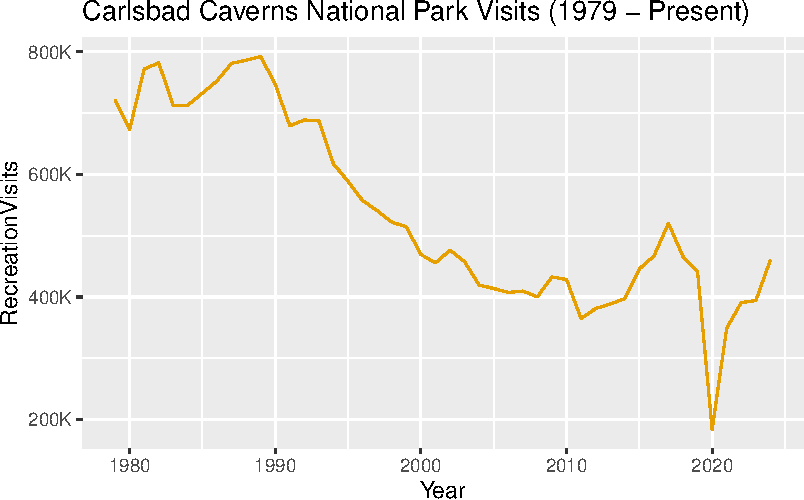
\includegraphics[keepaspectratio]{index_files/figure-pdf/unnamed-chunk-12-1.pdf}}

But after a little digging, we found out that in 2014 and 2015, Kobuk
Valley National Park actually didn't count visitors at all.

If we look at the
\href{https://irma.nps.gov/Stats/SSRSReports/Park\%20Specific\%20Reports/Monthly\%20Visitation\%20Comments\%20By\%20Park?Park=KOVA}{visitation
reports for Kobuk Valley in 2014}, they say that ``the park is
developing a new counting system and has made the decision not to report
visitor counts until the new system is in place.'' Though they didn't
count visitors at all, they still recorded a zero in those two years.
This hard number makes it seem conclusive, like there were truly zero
people who stepped onto the park lands in those years.

In 2015, John Quinley, the Alaska regional spokesperson for the NPS,
spoke with
\href{https://www.adn.com/outdoors/article/alaskas-little-visited-parks/2015/02/18/}{the
Anchorage Daily News about this issue}, and he admitted that ``it might
have been better if park statisticians had put something other than a
zero in the visitor box for 2014 --- say maybe a question mark.''

\begin{tcolorbox}[enhanced jigsaw, title=\textcolor{quarto-callout-tip-color}{\faLightbulb}\hspace{0.5em}{Activity 3}, opacityback=0, bottomtitle=1mm, left=2mm, coltitle=black, opacitybacktitle=0.6, breakable, arc=.35mm, colframe=quarto-callout-tip-color-frame, toprule=.15mm, rightrule=.15mm, colback=white, colbacktitle=quarto-callout-tip-color!10!white, leftrule=.75mm, toptitle=1mm, titlerule=0mm, bottomrule=.15mm]

Can you find evidence of people visiting Kobuk Valley National Park in
2014 and 2015? For more, see
\href{?tab=discussion-\%26-activities\#activity-3}{Activity 3}.

\end{tcolorbox}

\begin{tcolorbox}[enhanced jigsaw, title=\textcolor{quarto-callout-tip-color}{\faLightbulb}\hspace{0.5em}{Discussion Question 3}, opacityback=0, bottomtitle=1mm, left=2mm, coltitle=black, opacitybacktitle=0.6, breakable, arc=.35mm, colframe=quarto-callout-tip-color-frame, toprule=.15mm, rightrule=.15mm, colback=white, colbacktitle=quarto-callout-tip-color!10!white, leftrule=.75mm, toptitle=1mm, titlerule=0mm, bottomrule=.15mm]

Why would you or wouldn't you want to record a question mark in this
dataset? For more, see
\href{?tab=discussion-\%26-activities\#discussion-3}{Discussion Q 3}.

\end{tcolorbox}

The decision not to record visits in certain years seems reasonable on
its face, but we've also seen a \emph{lot} of parks in more
highly-frequented areas that, when faced with a similar situation, chose
to provide an estimate for a certain year based on average counts from
previous years, rather than simply declare that nobody visited.

When parks get more visits, they usually get more money, resources, and
staff. Once outfitted with more funding, resources, and staff, they can
usually attract and support even more visitors. By contrast, a dip in
visitation data can potentially lead to a cycle of stagnation or
decline. The choice to record zeros for Kobuk Valley NP in 2014 and 2015
was likely made out of a sense of scientific responsibility and
integrity. It's unclear how, if at all, this choice impacted the park.
But this example highlights how data collection decisions can have
real-world impacts, and how the people making these choices are often
aware of these impacts and must weigh trade-offs---not only from a
scientific or statistical perspective, but also from a social, economic,
political, and even personal perspective.

\subsection{Conclusion}\label{conclusion}

The NPS's visitation data is a valuable resource that gives us a glimpse
into the country's relationship with the National Parks---some of the
world's most precious natural resources---over the last 50 years. This
data is integral to the maintenance and growth of the parks, to
environmental conservation, to gateway communities, and to our
historical and sociological understanding. But the National Park visit
data, like all data, is also approximate and imperfect. As we have seen,
it is collected by imperfect devices, such as traffic counters that are
vulnerable to weather or malfunctioning. But even more importantly, it
is collected and shaped by people, people who not only count some of the
visits manually, but who also decide what counts as a visit, how to
count visits (e.g., to use this technology or that formula) and which
numbers to record when things don't go as planned. There are endless
interesting, important, and fun analyses that we can do with this visit
data, but to really make sense of it in any meaningful way, we need to
dig into and consider the people, context, and circumstances that shaped
it.

\subsection{References}\label{references}

\phantomsection\label{refs}
\begin{CSLReferences}{1}{0}
\bibitem[\citeproctext]{ref-alba_covid-19s_2022}
Alba, Charles, Bing Pan, Junjun Yin, William L. Rice, Prasenjit Mitra,
Michael S. Lin, and Yun Liang. 2022. {``{COVID}-19's Impact on
Visitation Behavior to {US} National Parks from Communities of Color:
Evidence from Mobile Phone Data.''} \emph{Scientific Reports} 12 (1):
13398. \url{https://doi.org/10.1038/s41598-022-16330-z}.

\bibitem[\citeproctext]{ref-beauchamp_beyond_2020}
Beauchamp, Toby. 2020. {``Beyond the {`{Pine} {Pig}'}: {Reimagining}
{Protection} Through the {US} {National} {Park} {Ranger}.''}
\emph{Radical History Review} 2020 (137): 96--118.
\url{https://doi.org/10.1215/01636545-8092798}.

\bibitem[\citeproctext]{ref-floyd_coming_2002}
Floyd, Myron F., and Cassandra Y. Johnson. 2002. {``Coming to {Terms}
with {Environmental} {Justice} in {Outdoor} {Recreation}: {A}
{Conceptual} {Discussion} with {Research} {Implications}.''}
\emph{Leisure Sciences}, January.
\url{https://doi.org/10.1080/01490400252772836}.

\bibitem[\citeproctext]{ref-spence_dispossessing_2000}
Spence, Mark David. 2000. \emph{Dispossessing the {Wilderness}: {Indian}
{Removal} and the {Making} of the {National} {Parks}}. New York; NY:
Oxford University Press.

\bibitem[\citeproctext]{ref-weber_why_2013}
Weber, Joe, and Selima Sultana. 2013. {``Why {Do} {So} {Few} {Minority}
{People} {Visit} {National} {Parks}? {Visitation} and the
{Accessibility} of {`{America}'s {Best} {Idea}'}.''} \emph{Annals of the
Association of American Geographers} 103 (3): 437--64.
\url{https://doi.org/10.1080/00045608.2012.689240}.

\end{CSLReferences}

\phantomsection\label{custom-footnotes}

\section{Explore the Data}

\subsection{Explore the Data}\label{explore-the-data}

\section{Exercises}

\subsection{Programming Exercises}\label{programming-exercises}

The National Park visitation data by year and month is well-suited for
teaching introductory data analysis, manipulation, and visualization
methods.

Based on our experience, the data is particularly useful for teaching
filter and groupby functions, where students can, for example, filter by
individual parks, states, or regions, or groupby and calculate summary
statistics for different parks, states, regions, or years.

The data is also useful for teaching basic and advanced visualization
methods, like creating line plots over time or customizing plot
aesthetics (e.g., abbreviating millions and thousands, altering axis
ranges).

When working on visualization methods, we often ask students to share
plots in a communal class forum, such as a shared Google Doc or
Discord/Slack. This approach can be effective for building community;
showcasing different ways of representing similar data; and enabling
instructors to identify common strengths or problems.

\section{R}

\phantomsection\label{exercise-posts-r}

\section{Python}

\phantomsection\label{exercise-posts-python}

\section{Discussion \& Activities}

\subsection{Activity 1}\label{activity-1-1}

\subsubsection{Devices Will Break}\label{devices-will-break}

It is inevitable that the devices that the National Park Service uses to
count visits to the parks ---~like induction loop counters installed on
the road ---~will break. But they will also get \emph{fixed} at
different rates, in different locations, as we could see in the case of
Crater Lake National Park (where a counter was fixed quickly) and
Carlsbad Caverns National Park (where a broken counter from 2019 still
has not been fixed).

There are many reasons for these disparities, but some of the big ones
might be geography and resources. The more remote a park, the harder it
is to get a repair team to it. The less-resourced a park, the lower the
likelihood they have on-site repair teams, or are prioritized by the
repair teams that can be dispatched.

With this in mind, look at the locations of the following parks. Suppose
that each one has an outage in their induction loop counter: which ones
would you expect to be fixed first, and why? Research the parks, and
rank them on a scale of 1 to 5 (1 being highest, and 5 being lowest) of
which would be fixed quickest.

\begin{longtable}[]{@{}lll@{}}
\toprule\noalign{}
Park & Priority (1-5) & Reason \\
\midrule\noalign{}
\endhead
\bottomrule\noalign{}
\endlastfoot
Acadia NP & & \\
Lassen Volcanic NP & & \\
Saguaro NP & & \\
Yosemite NP & & \\
Mammoth Cave NP & & \\
\end{longtable}

\subsection{Activity 2}\label{activity-2-1}

\subsubsection{Counting Procedures}\label{counting-procedures}

The National Park Service sometimes fills in missing data with hard
numbers or approximates data by applying special mathematical formulas.
This is necessary work, but it is also under-explained work.

To see this in action, go to
\href{https://irma.nps.gov/Stats/Reports/Park}{the NPS page that
documents park reports} and down the ``Visitor Use Counting Procedures''
PDF for three different parks.

How are the procedures for these three parks similar or different? What
kind of effect do you think this has on the resulting data? What do you
think is the best way of documenting this information and communicating
it to users of the data?

\subsection{Activity 3}\label{activity-3-1}

\subsubsection{Missing Evidence}\label{missing-evidence}

In 2014 and 2015, Kobuk Valley National Park reported that there were
zero visitors to the park.

Use publicly available internet
data---\href{https://www.flickr.com/}{Flickr photos}, Twitter posts,
etc.---to try and find evidence of people visiting the park. (Hint:
There is existing evidence to find!) Consider how you might use tags and
metadata categories to find what you're looking for.

Based on your findings, how do you think, differently, if at all, about
Kobuk Valley's decision to record zero visits and about alternative
methods for counting visits?

\subsection{Discussion Question 1}\label{discussion-question-1-1}

\subsubsection{Alternative Uses of the
Data}\label{alternative-uses-of-the-data}

We discussed some of the ways the National Park visit data is used. How
else might the data be used? How might it be used by artists,
historians, literary scholars, sociologists, or librarians?

\subsection{Discussion Question 2}\label{discussion-question-2-1}

\subsubsection{``Non-Recreation'' Visits}\label{non-recreation-visits}

Read through the
\href{https://www.nps.gov/subjects/socialscience/nps-visitor-use-statistics-definitions.htm}{full
list of the ``reportable non-recreation'' visits}, according to the NPS:

\begin{quote}
\begin{itemize}
\tightlist
\item
  Persons going to and from inholdings across significant parts of park
  land;
\item
  Commuter and other traffic using NPS-administered roads or waterways
  through a park for their convenience;
\item
  Trades-people with business in the park;
\item
  Any civilian activity a part of or incidental to the pursuit of a
  gainful occupation (e.g., guides);
\item
  Government personnel (other than NPS employees) with business in the
  park;
\item
  Citizens using NPS buildings for civic or local government business,
  or attending public hearings;
\item
  Outside research activities (visits and overnights) if independent of
  NPS legislated interests (e.g.~meteorological research).
\end{itemize}
\end{quote}

What are the potential consequences of considering these visits to be
\emph{non-recreation} vs.~\emph{recreation} visits?

\subsection{Discussion Question 3}\label{discussion-question-3-1}

\subsubsection{Recording Uncertainty}\label{recording-uncertainty}

In 2014 and 2015, Kobuk Valley National Park recorded zero visits, even
though they decided not to count visits at all. John Quinley, the Alaska
regional spokesperson for the NPS, spoke with
\href{https://www.adn.com/outdoors/article/alaskas-little-visited-parks/2015/02/18/}{the
Anchorage Daily News about this issue}, and he admitted that ``it might
have been better if park statisticians had put something other than a
zero in the visitor box for 2014 --- say maybe a question mark.''

Why would you or wouldn't you want to record a question mark in this
dataset? How would this impact a qualitative vs quantitative analysis of
the data?

What else could you use to record uncertainty? What would be the
potential consequences of that choice?




\end{document}
